
% Options for packages loaded elsewhere



%
\documentclass[twoside, man, a4paper,12pt, nofontenc]{apa7}

% deps for huxtable
\usepackage{array}
\usepackage{graphicx}
\usepackage{siunitx}
\usepackage{colortbl}
\usepackage{multirow}
\usepackage{hhline}
\usepackage{calc}
\usepackage{tabularx}
\usepackage{threeparttable}
\usepackage{wrapfig}
\usepackage{adjustbox}
\usepackage{hyperref}
\usepackage{fontenc}
\usepackage{polyglossia}

\usepackage{tabulary}
\usepackage{booktabs}
\usepackage[style=english]{csquotes}
\usepackage{hyperref}
\usepackage{xcolor}
\usepackage{sectsty}
\usepackage{tikz}
\usepackage{lineno}
\usepackage[section]{placeins}
\usepackage{caption}
\usepackage{floatrow}
%\usepackage[document]{ragged2e}
%\RaggedRightRightskip 0pt plus 4em

\usepackage{titlesec}


\setcounter{totalnumber}{1}

\floatsetup[figure]{capposition=top}
\floatsetup[table]{capposition=top}

%\linenumbers

\usepackage{amsmath}
\usepackage{unicode-math}

%\setmainfont[
%    BoldFont={Meta Pro Medium}
%]{Meta Pro}




\setmainfont[Numbers={Lining}]{Cochineal}
\setmathfont[Scale=MatchUppercase]{Latin Modern Math}
\setmathfont[range=\mathup/{num},Numbers=Lining]{Cochineal-Roman}
\setmathfont[range=it/{latin,Latin},Ligatures={NoCommon, NoDiscretionary, NoHistoric, NoRequired, NoContextual}]{Cochineal-Italic}

\newfontfamily\sansfont[Numbers=Lining]{Gill Sans}


\DeclareCaptionFormat{myformat}{#1#2\\\sansfont#3}
\DeclareCaptionFont{quack}{\sansfont}
\captionsetup[figure]{skip=5pt, font={up,small,quack}, labelsep=period, position=top, format=myformat, justification=justified, labelfont=sc}


\titleformat{\chapter}[display]
  {\huge\sansfont}{\chaptertitlename\ \thechapter}{20pt}{\Huge}
\titleformat*{\section}{\LARGE\sansfont}
\titleformat*{\subsection}{\Large\sansfont}

\shorttitle{Short Title Here}

\usepackage{amsfonts}

\newenvironment{cslreferences}%
  {}%
  {\par}


% Use upquote if available, for straight quotes in verbatim environments
\IfFileExists{upquote.sty}{\usepackage{upquote}}{}
\IfFileExists{microtype.sty}{% use microtype if available
  \usepackage[]{microtype}
  \UseMicrotypeSet[protrusion]{basicmath} % disable protrusion for tt fonts
}{}
\makeatletter
\@ifundefined{KOMAClassName}{% if non-KOMA class
  \IfFileExists{parskip.sty}{%
    \usepackage{parskip}
  }{% else
    \setlength{\parindent}{0pt}
    \setlength{\parskip}{6pt plus 2pt minus 1pt}}
}{% if KOMA class
  \KOMAoptions{parskip=half}}
\makeatother
\usepackage{newunicodechar}
\newunicodechar{✓}{\(\checkmark\)}
\newunicodechar{×}{\(×\)}



\usepackage{xcolor}
\IfFileExists{xurl.sty}{\usepackage{xurl}}{} % add URL line breaks if available
\IfFileExists{bookmark.sty}{\usepackage{bookmark}}{\usepackage{hyperref}}
\hypersetup{
  pdftitle={Revisiting the Stimulation-Rate-Dependent Pattern Mismatch Negativity},
  pdfauthor={Marc Pabst},
  pdflang={en-US},
  hidelinks,
  pdfcreator={LaTeX via pandoc}}
\urlstyle{same} % disable monospaced font for URLs

\usepackage{graphicx}
\makeatletter
\def\maxwidth{\ifdim\Gin@nat@width>\linewidth\linewidth\else\Gin@nat@width\fi}
\def\maxheight{\ifdim\Gin@nat@height>\textheight\textheight\else\Gin@nat@height\fi}
\makeatother
% Scale images if necessary, so that they will not overflow the page
% margins by default, and it is still possible to overwrite the defaults
% using explicit options in \includegraphics[width, height, ...]{}
%\setkeys{Gin}{width=\maxwidth,height=\maxheight,keepaspectratio}
% Set default figure placement to htbp
\makeatletter
\def\fps@figure{!tbp}
\makeatother
\setlength{\emergencystretch}{3em} % prevent overfull lines
\providecommand{\tightlist}{%
  \setlength{\itemsep}{0pt}\setlength{\parskip}{0pt}}
\setcounter{secnumdepth}{-\maxdimen} % remove section numbering
\makeatletter
\@ifpackageloaded{subfig}{}{\usepackage{subfig}}
\@ifpackageloaded{caption}{}{\usepackage{caption}}
\captionsetup[subfloat]{margin=0.5em}
\AtBeginDocument{%
\renewcommand*\figurename{Figure}
\renewcommand*\tablename{Table}
}
\AtBeginDocument{%
\renewcommand*\listfigurename{List of Figures}
\renewcommand*\listtablename{List of Tables}
}
\@ifpackageloaded{float}{}{\usepackage{float}}
\floatstyle{ruled}
\@ifundefined{c@chapter}{\newfloat{codelisting}{h}{lop}}{\newfloat{codelisting}{h}{lop}[chapter]}
\floatname{codelisting}{Listing}
\newcommand*\listoflistings{\listof{codelisting}{List of Listings}}
\makeatother


\newlength{\cslhangindent}
\setlength{\cslhangindent}{1.5em}
\newlength{\csllabelwidth}
\setlength{\csllabelwidth}{3em}
\newenvironment{CSLReferences}[3] % #1 hanging-ident, #2 entry sp
 {% don't indent paragraphs
  \setlength{\parindent}{0pt}
  % turn on hanging indent if param 1 is 1
  \ifodd #1 \everypar{\setlength{\hangindent}{\cslhangindent}}\ignorespaces\fi
  % set line spacing
  % set entry spacing
  \ifnum #2 > 0
  \setlength{\parskip}{#3\baselineskip}
  \fi
 }%
 {}
\usepackage{calc} % for \widthof, \maxof
\newcommand{\CSLBlock}[1]{#1\hfill\break}
\newcommand{\CSLLeftMargin}[1]{\parbox[t]{\maxof{\widthof{#1}}{\csllabelwidth}}{#1}}
\newcommand{\CSLRightInline}[1]{\parbox[t]{\linewidth}{#1}}
\newcommand{\CSLIndent}[1]{\hspace{\cslhangindent}#1}


\title{Revisiting the Stimulation-Rate-Dependent Pattern Mismatch
Negativity}
\author{Marc Pabst}
\date{}


\abstract{How does the brain process and represent successive sound in
close temporal proximity? By investigating mismatch negativity (MMN)
components, prior research (Sussman \& Gumenyuk, 2005; Sussman, Ritter
\& Vaughan, 1998) has suggested that temporal proximity plays an
important role in how sounds are represented in auditory memory. Here,
we investigate how predictability affects the election of mismatch
negativity components in auditory sequences consisting of two tones
(frequent tone A = 440 Hz, rare tone B = 494 Hz, fixed SOA 100 ms). In
the predictable condition, tones are presented in a fixed order whereas
in the unpredictable condition, standards and deviants are presented in
a pseudo-random order. We expect to find that B tones in the
unpredictable condition will elicit a significant MMN while B tones in
the predictable conditions will not. A repeating five-tone pattern was
presented at several stimulus rates (200, 400, 600, and 00 ms
onset-to-onset) to determine at what temporal proximity the five-tone
repeating unit would be represented in memory. The mismatch negativity
component of event-related brain potentials was used to index how the
sounds were organized in memory when participants had no task with the
sounds. Only at the 200-ms onset-to-onset pace was the five-tone
sequence unitized in memory. At presentation rates of 400 ms and above,
the regularity (a different frequency tone occurred every fifth tone)
was not detected and mismatch negativity was elicited by these tones in
the sequence. The results show that temporal proximity plays a role in
unitizing successive sounds in auditory memory. These results also
suggest that global relationships between successive sounds are
represented at the level of auditory cortices.}


\begin{document}

\maketitle


\renewcommand*\contentsname{}

\setcounter{tocdepth}{3}
\tableofcontents

\newpage

\hypertarget{introduction}{%
\section{Introduction}\label{introduction}}

Unraveling the mysteries of human perception might be one of the most
fascinating and difficult challenges in cognitive sciences. We usually
have little regard for this, but at every single moment, we achieve
something outstanding: By forming a coherent representation from the
tangled mess of external stimuli that reach our sensory organs, we make
sense of the outside world. In doing so and seemingly effortlessly, we
overcome complicated mathematical and philosophical problems. Recent
advances in emerging fields like computer vision and machine hearing
have provided a sense of how daunting these tasks can be---requiring
complex models that consume vast amounts of computational resources and
energy. What enables the brain to fulfill these functions with such ease
while consuming no more than the power equivalent of a lightbulb?

Over the centuries, many theories have been broad forward in an attempt
to answer these questions. While early philosophers like Aristotle
believed in the idea of direct or naïve realism (the idea that the
outside world is perceived directly), early modern scholars like John
Locke promoted the concept of indirect realism, which is highly
compatible with the assumption of representationalism in cognitive
science (perceptual experiences result from an internal representation
rather than directly from external objects). Among the first who
developed a consistent theory defining the rules followed by indirect
perception were the Gestalt psychologists of the early 20th century.
Wertheimer, Koffka, and Köhler hypothesized that Gestalt principles,
self-organizing rules on how individual elements should be grouped or
separated, guide perception. They based their principle on the
observation that humans perceive a global whole instead of just
collections of individual parts.

Much later, auditory scientists faced the same challenges described in
the first paragraph, but now in a very particular context: They were
puzzled by the brain's ability to convert small air pressure
fluctuations into actual auditory percepts. Somehow, the brain forms
meaningful perceptual experiences from what can only be described as a
busy mess of sound waves that originate from a plethora of different
sources differing in pitch, loudness, and spatial position. Known as the
\emph{cocktail party effect}
(\textbf{cherryExperimentsRecognitionSpeech1953?}), this problem was
compared to inferring the positions, shapes, and movements of motorboats
on a lake---just by observing how two nearby objects move up and down
the waves. Attempts to find answers to this perplexing question lead to
the development of auditory scene analysis (ASA). Not unlike the
concepts proposed by the Gestalt theorists six decades earlier,
(\textbf{bregman1990auditory?}) suggested that the brain uses so-called
\emph{streaming} and \emph{segregation} to form auditory objects from
rich spectro-temporal information. At its core, ASA relies on two
different categories of grouping, namely \emph{sequential} and
\emph{simultaneous} integration: Simultaneous integration (or vertical
integration) refers to the grouping of concurrent properties into one or
more separable auditory objects, a process informed by temporal cues
like common onset and offset, spectral and spatial characteristics.
Sequential integration (or horizontal integration), on the other hand,
describes how temporally distinct sounds are merged into one or multiple
coherently perceived streams (contrary to auditory objects in
simultaneous grouping, only one such stream can be actively perceived at
any time). While vertical and horizontal grouping can come to different
and therefore competing results, sequential grouping often takes
precedence over cues for simulations integration
(\textbf{bendixenPredictabilityEffectsAuditory2014?})

Often, the key to understanding such complex phenomena seems to lie in
learning about the most basic processing steps. In auditory research,
these steps usually come in the shape of very simple stimuli, often
consisting of nothing more than pure tones. Such stimuli were also the
first to be used in the auditory oddball paradigm, a now
well-established and robust paradigm extensively used in event-related
potential (ERP) studies (\textbf{squiresTwoVarietiesLonglatency1975?}).
In its basic form, participants are presented with a series of similar
tones or sounds (so-called \emph{standard} events), interrupted by rare
tones or sounds that differ in at least one feature (\emph{deviant}
events) from the more frequent ones. Strikingly, deviant events elicit
more extensive neural activity over sensory areas. This finding is known
as the mismatch negativity (MMN) component because when measured using
electroencephalography (EEG), a robust negative deflection can be
observed in the difference wave obtained by subtracting the response to
standard events from the response to deviant events. Negativity is
strongest in the frontotemporal area of the scalp, with a peak latency
ranging from 100 to 250 ms after stimulus onset. The elicitation of an
MMN is not restricted to the repetition of physically identical stimuli
but can also be observed when deviant events are complex, e.g., when
abstract auditory regularities are violated (Paavilainen, 2013). The
regularities can come in the form of relationships between two (Saarinen
et al., 1992) or multiple tones (Alain et al., 1994; Nordby et al.,
1988; Schröger et al., 1996).

Interestingly, implications from MMN components are highly compatible
with another prevalent theory of perception, namely the idea that
perception is not (only) a stimulus-driven bottom-up process, but is
informed by internal predicitons of some kind. In spite of their recent
popularity, ideas of this nature have been around a long time and
famously trace back to the physiologist Hermann von Helmholtz. Gregory's
\enquote{perceptions as hypotheses}-sentiment is simmilarly well-known.
Most recently, this notion has been introduced in a theory knows as
(hierarchical) predictive coding. Predictive coding specifically
suggests that at every processing state, predictions from so-called
\emph{probabilistic generative models} and sensory input are compared
continuously, and only their difference, termed \emph{prediction error},
is propagated. MMN responses have been proposed as an index of
prediction error (\textbf{wacongneEvidenceHierarchyPredictions2011?}).
Although other interpretations exist (e.g.,
\textbf{mayMismatchNegativityMMN2010?}), the MMN is frequently
interpreted as a marker of expectation violations---a notion
particularly emphasising the role that predicitons plays in perception
(e.g., István Winkler, 2007).

An interesting situation arises when concurrent predictive clues exist.
Following this idea, E. Sussman et al. (1998) presented participants
with a sequence of frequent pure tones and rare pitch deviants while
reading a book of their choice. Tones were arranged in a predictable
five-tone pattern consisting of four standard tones and one deviant
(i.e., A-A-A-A-B-A-A-A-A-B, '\enquote*{-}' indicating silence between
the tones). ERPs to A and B tones were compared for rapid (SOA of 100
ms) and slow (SOA of 1300 ms) stimulation rates. The 100 ms SOA
condition also included a control condition in which tone order was
pseudo-randomized (e.g., A-A-A-B-A-B-A-A-A) without altering deviant
probability (\(p_B = .20\)). When tones are presented randomly, only
their relative frequency of occurrence carries value for predicting the
pitch of the next tone. This, we refer to as \emph{proportional
regularity}. However, in an ordered presentation, a sequence of four
standard tones is always followed by one deviant tone. Thus,
understanding this relationship should allow for \emph{perfect
prediction} in which all deviant tones are expected with near-absolute
certainty. We call this regularity a \emph{pattern regularity}. Provided
the underlying mechanism can incorporate such information, the
processing of the pitch deviants should correspond with that of standard
tones, and therefore no MMN would be elicited. Interestingly, in the
case of Sussman et al., MMNs were only elicited if tone presentation was
slow and predictable or fast and random, but not when predictable tones
were presented rapidly. In a subsequent study, E. S. Sussman \& Gumenyuk
(2005) used the same pattern at different SOAs (200 ms, 400 ms, and 800
ms). Similar to their previous study, grouped presentation at 400 ms and
800 ms SOA elicited an MMN response, while at a stimulation rate of 200
ms, evidence for such a deflection was absent. Sussman et al.~attributed
this observation to sensory memory limitations. That is, only when
auditory memory can accommodate enough repetitions of the five-tone
pattern; the brain can integrate tones into a coherent representation
allowing for accurate predictions of deviant tones. This, in turn, would
explain the absence of MMNs in the fast presentation condition. Based on
this, they argued that while true for fast presentation rates with SOAs
up to 200 ms, for longer SOAs, pattern durations would be too long, and
thus representations would exceed sensory memory capacity.

In a recent in-class replication study,
(\textbf{scharfPredictableChangesFastpacedinprep?}) presented
participants with the same stimuli as Sussmann in a very similar
experimental setting. Their study only differed in that participants
were given a simple task in which they had to count visual targets
instead of reading a book of their choice. Surprisingly, while
descriptive results were compatible with those of Sussmann et al.,
pairwise comparisons revealed no significant effect when comparing
deviant and standard tones for both the \emph{random} and the
\emph{predictable} condition. Further Bayesian analysis remained largely
inconclusive, providing only \emph{anecdotal} evidence in favor of such
an effect for \emph{random} presentation and \emph{moderate} evidence
for its absence in the \emph{predictable} condition. In the face of the
replication crisis, many scientists have become painfully aware of the
importance of replicability (\textbf{ioannidisWhyMostPublished2005?}).
Exact or quasi-exact replication studies that try to match the original
study's experimental conditions as closely as possible are regarded as
the gold standard of science (\textbf{popperLogikForschungZur1935?};
\textbf{jasnyAgainAgainAgain2011?}). However, replications that extend,
change, or optimize materials or methods of the original work also offer
valuable insight. This kind of replication is known as conceptual
(\textbf{schmidtShallWeReally2009?}) and refers to using of different
methods to repeat the test of a hypothesis or experimental result.

This thesis seeks to replicate the findings by Sussman et al.~It largely
follows the procure laid out by E. S. Sussman \& Gumenyuk (2005).
However, it deviates from the original design in some critical
aspects.First, the aforementioned five-tone patterns are presented in
both the~\emph{predictable}~condition and in the~\emph{random}~context.
That is, pseudo-random order will be deliberately broken by occasionally
presenting B-A-A-A-A-B-patterns. In particular, this will ensure that
the local history of B-tones in the \emph{random} condition is
comparable to that in the \emph{predictable} condition. Secondly, B
tones are compared exclusively with their preceding A tones. Lastly, a
small number of A-A-A-A-B will be replaced by A-A-A-A-A sequences in
both conditions, allowing the comparison of physically identical tones
in different contexts. The advantages of this design are discussed in
more detail in the following paragraphs. A pre-registration covering
data collection, processing, and analysis is available at
https://osf.io/cg2zd/. Deviations from this pre-specified plan and
further exploratory analyses are explicitly reported.

E. S. Sussman \& Gumenyuk (2005) interpretation of the original results
suggests that at fast stimulation rates (200 ms and faster),
pattern-based regularities take precedence over proportion-based
regularities. If this is indeed true, B-tones in the \emph{predictable}
condition should not be considered a \emph{mismatch} and thus should not
elict an MMN response. In contrast, since there is no way to reliably
predict B-tones in the~\emph{random}~condition, these tones would still
be considered~\emph{deviant}~events and are therefore expected to
generate an MMN. On the other hand, when an A tone replaces a
predictable B tone, one would expect an MMN, despite tones are
physically identical. Specifically, hypotheses are formulated in regards
to the ERPs elicited by the 5th tone in the five-tone sequence
(A-A-A-A-\textbf{B} or A-A-A-A-\textbf{A}; boldface marks tone of
interest) compared to the 4th tone in that sequence (A-A-A-\textbf{A}-X,
\enquote{X} marking either an A or an B tone). Hypotheses can be
summarized as follows:

\hypertarget{pattern-regularities}{%
\paragraph{Pattern regularities}\label{pattern-regularities}}

If Sussman's intepreation holds, one expects i) negativity in the N1/MMN
time domain (about 100-200 ms after tone onset) for deviations in the
BAAAA\emph{B} sequence in the \emph{random} condition, since B tones
violate the \emph{proportional regularity}, ii) one expects no evidence
for such an effect (or evidence favoring \(\mathcal{H_0}\) i.e., that
there is no effect) in the \emph{predictable} context since more
informative higher-order predictions based on \emph{pattern regularity}
are not violated, and iii) the difference waves should differ
significantly. Also, the comparison between the 5th A tone and the
proceeding A tone (A-A-A-\textbf{A}-X vs.~A-A-A-A-\textbf{A}) should be
consiered a \emph{mismatch} and is therefore expected to elicit a
significant MMN response.

\hypertarget{proportional-regularities}{%
\paragraph{Proportional regularities}\label{proportional-regularities}}

If, however, no \emph{pattern regularity} is extracted,~B-tones should
continuously result in an MMN regardless of presentation context since
the predictive value of the~\emph{proportional regularity}~does not
differ between conditions. When prsenting A tones at the 5th position,
no MMN should occur. Also, difference waves should not differ.

\hypertarget{pattern-regularities-and-proportional-regularities}{%
\paragraph{Pattern regularities and proportional
regularities}\label{pattern-regularities-and-proportional-regularities}}

As a third possibility, the brain might use \emph{proportional
regularities} and \emph{pattern regularities} concurrently, resulting in
negativity following B-tones in either condition. Fifth-posiiton A tones
should consitute an expectation violation and should therefore results
in a negative deflection.

\newpage

\hypertarget{methods-and-materials}{%
\section{Methods and Materials}\label{methods-and-materials}}

\hypertarget{participants}{%
\subsubsection{Participants}\label{participants}}

All participants were recruited at the Institute of Psychology at the
University of Leipzig and reported good general health, normal hearing,
and normal or corrected-to-normal vision. Written informed consent was
obtained before the experiment. Participants were blinded to the purpose
of the experiment and received compensation in course credit or money.

For the 100 ms presentation rate, data were collected from twenty
participants (2 males, average age 22.3 yrs., \(SD=6.46\), range 18 - 41
yrs.). The sample for the 150 ms presentation rate consisted of
twenty-three psychology undergraduate students (2 males, average age
22.6 yrs., \(SD=5.57\), range 18 - 42). Here, participants were also
asked to provide information regarding their prior musical training: at
the time of the survey, approximately one-third (34.8\%) of participants
engaged in musical activities, while 8.7\% had no prior musical
experience.

\hypertarget{procedure-and-stimuli}{%
\subsubsection{Procedure and Stimuli}\label{procedure-and-stimuli}}

\begin{figure}
\centering
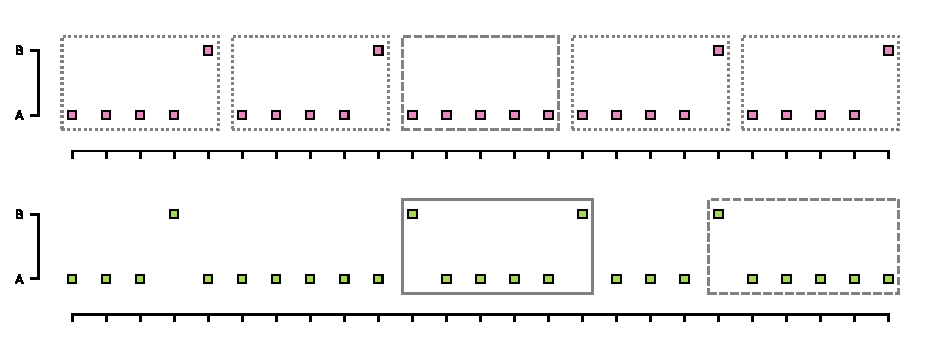
\includegraphics{figures/fig_tones.pdf}
\caption{Caption}
\end{figure}

Participants sat in a comfortable chair in a sound-insulated chamber.
The experimental setup was practically identical to that of Sussman et
al.; however, instead of reading a book, subjects were asked to direct
their attention to a self-selected movie. Movies were presented with
subtitles but without sound. Commercially available software (MATLAB
R2014a; The MathWorks Inc, Natick, MA) in conjunction with the
Psychophysics Toolbox extension (version 3.0.12,
\textbf{brainardPsychophysicsToolbox1997?};
\textbf{kleinerWhatNewPsychtoolbox32007?}) was used to control stimulus
presentation. Stimuli consisted of pure sinusoidal tones with a duration
of 50 ms (including a 10 ms cosine on/off ramp), presented isochronously
at a stimulation onsets asynchrony (SOA) of 100 ms or 150 ms,
respectively. Tone presentation was blocked and participants had the
option to take a break after each block. Blocks contained 820 frequent
440 Hz tones (\enquote{A} tones) and 180 infrequent 449 Hz tones
(\enquote{B} tones), delivered binaurally using Sennheiser HD-25-1 II
headphones at 70 dB. For the 100 ms condition, participants were
presented with 40 blocks, while 20 blocks were presented in the 150 ms
condition. In one-half of the blocks, tones occurred in pseudo-random
order (e.g., A-A-A-B-A-B-A\}, \emph{random} condition) while in the
other half, tone presentation followed a simple pattern in which a
five-tone-sequence of four frequent tones and one infrequent tone (i.e.,
A-A-A-A-B) was repeated cyclically (\emph{predictable} condition). Block
order was counterbalanced across participants. Additionally, A tones
replaced 10\% of designated (infrequent) B tones, resulting in sporadic
five-tone sequences consisting solely of A tones (i.e., A-A-A-A-A), thus
violating the \emph{pattern regularity}. To assure comparability of
local histories between tones of interest in both conditions,
pseudo-randomly arranged tones were interspersed with sequences matching
those from the predictable condition (i.e., B-A-A-A-A-B and
B-A-A-A-A-A). Care was taken that sequences in the \emph{random
condition} were always sepearated by at least five pseudo-random tones
and that A-A-A-A-A-patterns were always seperated by at least two
A-A-A-A-B-patterns. A total of 2000 tones at 150 ms SOA or 4000 tones at
100 ms SOA were delivered to each participant resulting in a total
duration (exluding potential breaks) of 1 hour and 20 minutes (100 ms
SOA) and 50 minutes (150 ms SOA), respectively.

\hypertarget{data-acquisition}{%
\subsubsection{Data Acquisition}\label{data-acquisition}}

Electrophysiological data were recorded from active
silver-silver-chloride (\emph{Ag}-\emph{AgCl}) electrodes using an
ActiveTwo amplifier system (BioSemi B.V., Amsterdam, The Netherlands). A
total of 39 channels were obtained using a 32-electrode-cap and seven
external electrodes. Scalp electrode locations conformed to the
international 10--20 system. Horizontal and vertical eye movement was
obtained using two bipolar configurations with electrodes placed around
the lateral canthi of the eyes as well as above and below the right eye.
Additionally, three electrodes were placed on the tip of the nose and at
the left and right mastoid sites. Data were sampled at 512 Hz and
on-line low-pass filtered at 1000 Hz.

\hypertarget{analysis-pipeline}{%
\subsubsection{Analysis Pipeline}\label{analysis-pipeline}}

Data prepossessing was implemented using a custom pipeline based on the
\emph{MNE Python} software package (Gramfort, 2013) using \emph{Python
3.7}. Ccomputations were partly carried out on a cluster operated by the
University Computation Center of the University of Leipzig. Code used in
this thesis is publicly available at
\url{https://github.com/marcpabst/xmas-oddballmatch}.

First, EEG data were subjected to the ZapLine procedure (de Cheveigné,
2020) to remove line noise contamination. A fivefold detection
procedure, as described by Bigdely-Shamlo et al. (2015) was then used to
detect and subsequently interpolate bad channels. Namely, this included
detecting channels that contained prolonged segments with very small
values (i.e., flat channels), the exclusion of channels based on robust
standard deviation (deviation criterion), unusually pronounced
high-frequency noise (noisiness criterion), and the removal of channels
that were poorly predicted by nearby channels (correlation criterion and
predictability criterion). Channels considered bad by one or more of
these methods were removed and interpolated using spherical splines
(Perrin et al., 1989). Electrode locations for interpolations were
informed by the BESA Spherical Head Model.

For independent component analysis (ICA), a 1-Hz-high-pass filter (134th
order hamming-windowed FIR) was applied (Irene Winkler et al., 2015).
Artifact Subspace Reconstruction (ASR, Mullen et al., 2015) was used to
identify and remove parts of the data with unusual noise characteristics
(bursts). ICA was then carried out using the \emph{Picard} algorithm
(Ablin et al., 2018, 2017) on principal-component-analysis--whitened
(PCA) data. PCA was also used for dimensionality reduction to avoid
rank-deficiency when extracting components from data with one or more
interpolated channels. The EEGLAB (version 2020.0, Delorme \& Makeig,
2004) software package and the IClabel plugin (version 1.2.6,
Pion-Tonachini et al., 2019) were used to classify estimated components
automatically. Only components clearly classified (i.e., confidence
above 50\%) resulting from either eye movement, muscular, or heartbeat
activity were zeroed-out before applying the mixing matrix to unfiltered
data.\footnote{Pre-registration states that ICA components should be
  reviewed by two experianced analysts. It should be noted that this
  procedure deviated from the pre-registration in that it was fully
  automated.}

In line with recommendations from Widmann et al. (2015) and de Cheveigné
\& Nelken (2019), a finite impulse response (FIR) bandpass filter from
0.1 Hz to 40 Hz (Hamming window, 0.1 Hz lower bandwidth, 5 Hz upper
bandwidth, 0.0194 passband ripple, and 53 dB stopband attenuation) was
applied. Continuous data were epoched into 400 ms long segments around
stimulus onsets, including a 100 ms pre-stimulus interval. No baseline
correction was applied, and segments exceeding a peak-to-peak voltage
difference of 100 µV were removed. On average, (TODO) epochs were
dopped. No dataset met the pre-registered exclusion criterion of less
than 100 valid trials per condition; thus, data from all participants
(20 for 100 ms presentation rate and 23 for 150 ms presentation rate)
were included in the analysis.

\hypertarget{statistical-analysis}{%
\subsubsection{Statistical Analysis}\label{statistical-analysis}}

Statistical analysis was carried out using the \emph{R} programming
language (version 3.2, The R Core Team) using the \emph{rstatix} package
(version 2.0, \textbf{kassambaraRstatixPipefriendlyFramework2020?}).

Calculation of the dependant variable followed the original study's
procedure in averaging amplitudes in a time window extending ±25 ms
around the expected peak of negativity. Specifically, this peak was
obtained by subtracting the average ERP following the A tones from the
average ERP following B tones in the \emph{random condition} for both
presentation rates separately. To compute mean amplitudes, ERPs to 4th
position A tones (A-A-A-\textbf{A}-X, \textbf{boldface} indicates the
tone of interest) and B tones (A-A-A-A-\textbf{B}) were averaged
separately for both the \emph{random} and the \emph{predictable}
\emph{condition}. For the \emph{random condition}, only tones presented
as part of a sequence matching the patterns from the \emph{predictable}
condition were included in the analysis.

In accordance with the original analysis by E. S. Sussman \& Gumenyuk
(2005), mean amplitudes for frontocentral electrodes (pooled FZ, F3, F4,
FC1, and FC2) and the two mastoid positions (pooled M1 and M2) were
averaged separately. Then, for both SOAs, independent two-way
repeated-measures analyses of variance (ANOVA) with factors
\emph{condition} (levels \emph{predictable} and \emph{random}),
\emph{stimulus type} (levels \emph{A tone} and \emph{B tone}), and their
interaction were calculated. Following this, significant interaction
effects were further investigated using post-hoc \emph{t}-tests.

Going beyond the original study and extending the pre-registered
procedure, Bayesian analysis was conducted for ANOVA posthoc
comparisons. As mentioned above, traditional null hypothesis testing has
some limitations that are often overlooked, leading to incorrect
conclusions drawn from results. For example, failure to reject the null
hypothesis can usually not be interpreted as evidence in favor of
\(\mathcal{H_0}\) (e.g., \textbf{aczelQuantifyingSupportNull2018?};
\textbf{meehlTheoreticalRisksTabular1978?};
\textbf{kirkPracticalSignificanceConcept1996?};
\textbf{goodmanDirtyDozenTwelve2008?}). Similarly, p-values might
exaggerate evidence against \(\mathcal{H_0}\) (that is, observed data
might be more likely under \(\mathcal{H_0}\) than under
\(\mathcal{H_1}\) even tough \(\mathcal{H_0}\) is rejected, e.g.,
\textbf{hubbardWhyValuesAre2008?};
\textbf{rouderBayesianTestsAccepting2009?};
\textbf{wagenmakersBayesianInferencePsychology2018?};
\textbf{sellkeCalibrationValuesTesting2001?}). Conversely, Bayesian
hypothesis testing using Bayes factors can provide an intuitive way to
compare observed data's likelihood under the null hypothesis versus the
alternative hypothesis
(\textbf{wagenmakersPracticalSolutionPervasive2007?}), thereby making it
possible to evaluate the null hypothesis:
\(BF_{10} = \frac{Pr(data|\mathcal{H}_0)}{Pr(data|\mathcal{H}_1)}\).
Here, this approach was applied in agreement with the concept described
by (\textbf{rouderBayesianTestsAccepting2009?}) as an alternative to
classical frequentist paired \emph{t}-tests. Following their sentiment,
Bayes factors for within-participant differences \(y_i\) were computed
assuming \(\mathcal{H_0}: y_i \sim Normal(0, \sigma^2)\) and
\(\mathcal{H_1}: y_i \sim Normal(\delta, \sigma^2)\);
\(\delta \sim Cauchy(0, 1/\sqrt{2})\). A Jeffreys prior was used for the
variance \(\sigma^2\) in both models:
\(p(\sigma^2) \propto 1/\sigma^2\). Calculations were performed using
the Hamiltonian Monte Carlo method implemented in \emph{Stan} (version
2.25, \textbf{carpenterStanProbabilisticProgramming2017?}) and
\emph{RStan} (\textbf{standevelopmentteamRStanInterfaceStan2020?}).

Finally, the relationship between epoch number and the reliability of
the estimate was analyzed by drawing random subsamples of different
sizes from both data sets and calculating split-half reliability
employing the Spearman--Brown approach. Thus, single-trial responses for
all A and B tones in the predictable condition were randomly shuffled.
Then, \(100, 200, ..., N_{max}\)
(\(N_{max, 100ms} = 2500, N_{max, 150ms}=1300\)) epochs were drawn,
randomly assigned to one of two halves, and averaged separately for A
and B tones. Then, split-half reliability was calculated based on the
mean amplitude in the MMN latency window as defined above. The
Spearman--Brown prophecy formula\footnote{as given by
  \({\rho}_{xx'} = \frac{2{\rho}_{12}}{1+{\rho}_{12}}\), where
  \({\rho_{12}}\) is the Pearson correlation coefficient between the two
  halfes.} (\textbf{brownEXPERIMENTALRESULTSCORRELATION1910?};
\textbf{spearmanCorrelationCalculatedFaulty1910?}) was used to obtain
corrected reliability. This procedure was repeated 100 times for each
\(N\), and split-half-reliabilities obtained as such were subsequently
averaged.

\newpage

\hypertarget{results}{%
\section{Results}\label{results}}

\begin{figure}
\hypertarget{fig:fronto}{%
\centering
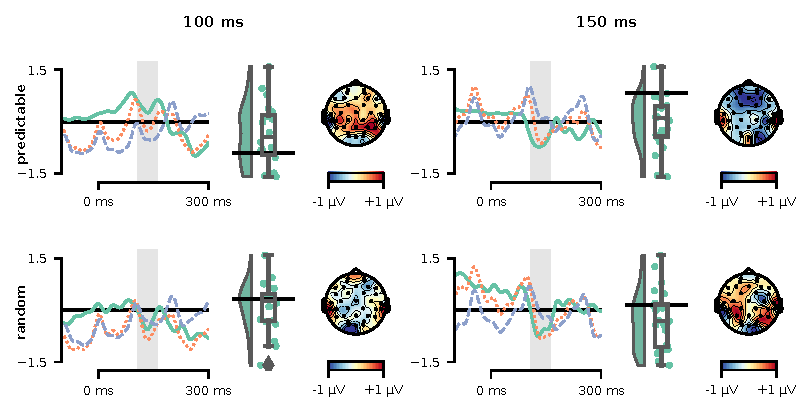
\includegraphics{figures/fig_fronto.pdf}
\caption{ERP grand averages (pooled FZ, F3, F4, FC1, and FC2 electrode
locations) for an SOA of 100 ms (left) and 150 ms (right), for A tones
(A-A-A-\textbf{A}-X, blue dashed lines) and B tones (A-A-A-A-\textbf{B},
orange dashed line) and their difference (B - A, green solid line).
Upper panels show ERPs for tones presented in a predcitable pattern
(\emph{predcitable condition}) while lower panels show ERPs for tones
presented in pseudo-random order (\emph{random condition}). Shaded area
marks MMN latency window (110 ms to 160 ms) used to calculate the
distribution of amplitude differences across particpants (middle of each
panel) and the difference of topographic maps averaged over the same
interval (right of each panel).}\label{fig:fronto}
}
\end{figure}

Fig.~\ref{fig:fronto} displays grand averages of event-related
potentials (ERP) at pooled FZ, F3, F4, FC1, and FC2 electrode locations
to A tones (A-A-A-\textbf{A}-X), B tones (A-A-A-A-\textbf{B}), and their
difference (B tone minus A tone) for both 100 ms (left panel) and 150 ms
(right panel) SOAs. The top half of each panel shows ERPs in the
\emph{predictable condition} while the lower half depicts ERPs in the
\emph{random condition}. Clearly visible rhythms result from fast
presentation frequencies and illustrate the considerable overlap between
neighboring tones. Panels also show the distribution of mean amplitude
differences in the MMN latency window across participants and the
difference of scalp topographies. Similarly, waveforms and mean
amplitude difference distributions at pooled mastoid sites are shown in
fig.~\ref{fig:mastoids}.

\begin{figure}
\hypertarget{fig:mastoids}{%
\centering
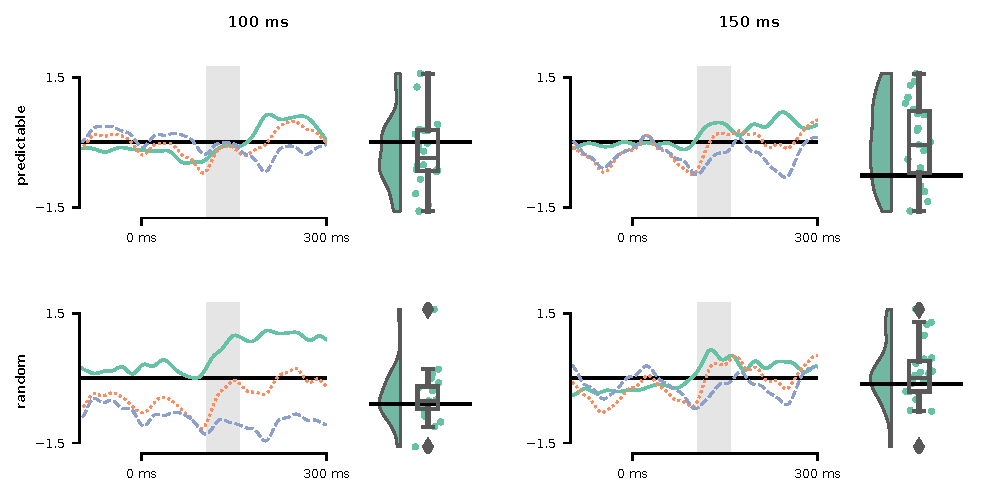
\includegraphics{figures/fig_mastoids.pdf}
\caption{ERP grand averages (pooled M1, M2 electrode locations) for an
SOA of 100 ms (left) and 150 ms (right), for A tones
(A-A-A-\textbf{A}-X, blue dashed lines) and B tones (A-A-A-A-\textbf{B},
orange dashed line) and their difference (B - A, green solid line).
Upper panels show ERPs for tones presented in a predcitable pattern
(\emph{predcitable condition}) while lower panels show ERPs for tones
presented in pseudo-random order (\emph{random condition}). Shaded area
marks MMN latency window (110 ms to 160 ms) used to calculate the
distribution of amplitude differences across
particpants.}\label{fig:mastoids}
}
\end{figure}

The MMN latency window was determined to range from 108 ms to 158 ms
ofter stimilus onset for 100 ms SOA and from 104 ms to 154 ms after
stimulus onset for 150 ms SOA. Mean amplitudes from the so-defined
interval are shown in Table 1. Descriptively, mean amplitudes at pooled
frontocentral electrode locations were more negative for randomly
presented B tones than for randomly presented A tones, regardless of
presentation rate (100 ms: \(\Delta M = -0.361 \: \mu V\); 150 ms:
\(\Delta M = -0.518 \: \mu V\)). A simmilar observation could be made
for predictable tones presented at 150 ms SOA
(\(\Delta M = -0.588 \: \mu V\)), Strikingly however, B tones presented
at an SOA of 100 ms seemed to elicit more positive responses than
associated A tones (\(\Delta M = 0.379 \: \mu V\)).

Statistical analysis was carried out by separate two-way
repeated-measures analyses of variance (ANOVA, Table 2). For the 100 ms
SOA presentation, ANOVA results for the frontocentral electrode cluster
revealed a significant effect of the interaction term (\emph{condition}
x \emph{stimulus type}; \(F(1,19) = 17.00\), \(p = 0.0006\)). For slower
tone presentation (150 ms SOA), ANOVA results suggested a main effect of
factor \emph{stimulus type} for both frontocentral (\(F(1,22) = 21.62\),
\(p < .001\)) and mastoid electrodes (\(F(1,22) = 6.26\),
\(p = 0.0200\)). ANOVAs for the comparison between the 4th A tone and
the 5th A tone (A-A-A-\textbf{A}-X versus A-A-A-A-\textbf{A}; Table 2)
did not result in any significant effects.


  \providecommand{\huxb}[2]{\arrayrulecolor[RGB]{#1}\global\arrayrulewidth=#2pt}
  \providecommand{\huxvb}[2]{\color[RGB]{#1}\vrule width #2pt}
  \providecommand{\huxtpad}[1]{\rule{0pt}{#1}}
  \providecommand{\huxbpad}[1]{\rule[-#1]{0pt}{#1}}

\begin{table}[ht]
\begin{centerbox}
\begin{threeparttable}
\captionsetup{justification=centering,singlelinecheck=off}
\caption{Results of the 2-way ANOVA (condition x stimulus type) for repeated measures. Only fronto included.}
 \setlength{\tabcolsep}{0pt}
\begin{tabular}{l l l l l l l l l}


\hhline{>{\huxb{0, 0, 0}{0.4}}->{\huxb{0, 0, 0}{0.4}}->{\huxb{0, 0, 0}{0.4}}->{\huxb{0, 0, 0}{0.4}}->{\huxb{0, 0, 0}{0.4}}->{\huxb{0, 0, 0}{0.4}}->{\huxb{0, 0, 0}{0.4}}->{\huxb{0, 0, 0}{0.4}}->{\huxb{0, 0, 0}{0.4}}-}
\arrayrulecolor{black}

\multicolumn{1}{!{\huxvb{0, 0, 0}{0}}l!{\huxvb{0, 0, 0}{0}}}{\huxtpad{6pt + 1em}\raggedright \hspace{0pt} \rotatebox{90}{\textbf{}} \hspace{6pt}\huxbpad{6pt}} &
\multicolumn{1}{l!{\huxvb{0, 0, 0}{0}}}{\huxtpad{6pt + 1em}\raggedright \hspace{6pt} \rotatebox{90}{\textbf{}} \hspace{6pt}\huxbpad{6pt}} &
\multicolumn{1}{l!{\huxvb{0, 0, 0}{0}}}{\huxtpad{6pt + 1em}\raggedright \hspace{6pt} \textbf{Effect} \hspace{6pt}\huxbpad{6pt}} &
\multicolumn{1}{r!{\huxvb{0, 0, 0}{0}}}{\huxtpad{6pt + 1em}\raggedleft \hspace{6pt} \textbf{DFn} \hspace{6pt}\huxbpad{6pt}} &
\multicolumn{1}{r!{\huxvb{0, 0, 0}{0}}}{\huxtpad{6pt + 1em}\raggedleft \hspace{6pt} \textbf{DFd} \hspace{6pt}\huxbpad{6pt}} &
\multicolumn{1}{r!{\huxvb{0, 0, 0}{0}}}{\huxtpad{6pt + 1em}\raggedleft \hspace{6pt} \textbf{F} \hspace{6pt}\huxbpad{6pt}} &
\multicolumn{1}{r!{\huxvb{0, 0, 0}{0}}}{\huxtpad{6pt + 1em}\raggedleft \hspace{6pt} \textbf{p} \hspace{6pt}\huxbpad{6pt}} &
\multicolumn{1}{l!{\huxvb{0, 0, 0}{0}}}{\huxtpad{6pt + 1em}\raggedright \hspace{6pt} \textbf{p$<$.05} \hspace{6pt}\huxbpad{6pt}} &
\multicolumn{1}{r!{\huxvb{0, 0, 0}{0}}}{\huxtpad{6pt + 1em}\raggedleft \hspace{6pt} \textbf{ges} \hspace{0pt}\huxbpad{6pt}} \tabularnewline[-0.5pt]


\hhline{>{\huxb{0, 0, 0}{0.4}}->{\huxb{0, 0, 0}{0.4}}->{\huxb{0, 0, 0}{0.4}}->{\huxb{0, 0, 0}{0.4}}->{\huxb{0, 0, 0}{0.4}}->{\huxb{0, 0, 0}{0.4}}->{\huxb{0, 0, 0}{0.4}}->{\huxb{0, 0, 0}{0.4}}->{\huxb{0, 0, 0}{0.4}}-}
\arrayrulecolor{black}

\multicolumn{1}{!{\huxvb{0, 0, 0}{0}}l!{\huxvb{0, 0, 0}{0}}}{} &
\multicolumn{1}{l!{\huxvb{0, 0, 0}{0}}}{} &
\multicolumn{1}{l!{\huxvb{0, 0, 0}{0}}}{\huxtpad{6pt + 1em}\raggedright \hspace{6pt} Condition \hspace{6pt}\huxbpad{6pt}} &
\multicolumn{1}{r!{\huxvb{0, 0, 0}{0}}}{\huxtpad{6pt + 1em}\raggedleft \hspace{6pt} 1 \hspace{6pt}\huxbpad{6pt}} &
\multicolumn{1}{r!{\huxvb{0, 0, 0}{0}}}{\huxtpad{6pt + 1em}\raggedleft \hspace{6pt} 19 \hspace{6pt}\huxbpad{6pt}} &
\multicolumn{1}{r!{\huxvb{0, 0, 0}{0}}}{\huxtpad{6pt + 1em}\raggedleft \hspace{6pt} 0.137 \hspace{6pt}\huxbpad{6pt}} &
\multicolumn{1}{r!{\huxvb{0, 0, 0}{0}}}{\huxtpad{6pt + 1em}\raggedleft \hspace{6pt} .715 \hspace{6pt}\huxbpad{6pt}} &
\multicolumn{1}{l!{\huxvb{0, 0, 0}{0}}}{\huxtpad{6pt + 1em}\raggedright \hspace{6pt}  \hspace{6pt}\huxbpad{6pt}} &
\multicolumn{1}{r!{\huxvb{0, 0, 0}{0}}}{\huxtpad{6pt + 1em}\raggedleft \hspace{6pt} 0.002~~~ \hspace{0pt}\huxbpad{6pt}} \tabularnewline[-0.5pt]


\hhline{}
\arrayrulecolor{black}

\multicolumn{1}{!{\huxvb{0, 0, 0}{0}}l!{\huxvb{0, 0, 0}{0}}}{} &
\multicolumn{1}{l!{\huxvb{0, 0, 0}{0}}}{} &
\multicolumn{1}{l!{\huxvb{0, 0, 0}{0}}}{\huxtpad{6pt + 1em}\raggedright \hspace{6pt} StimulusType \hspace{6pt}\huxbpad{6pt}} &
\multicolumn{1}{r!{\huxvb{0, 0, 0}{0}}}{\huxtpad{6pt + 1em}\raggedleft \hspace{6pt} 1 \hspace{6pt}\huxbpad{6pt}} &
\multicolumn{1}{r!{\huxvb{0, 0, 0}{0}}}{\huxtpad{6pt + 1em}\raggedleft \hspace{6pt} 19 \hspace{6pt}\huxbpad{6pt}} &
\multicolumn{1}{r!{\huxvb{0, 0, 0}{0}}}{\huxtpad{6pt + 1em}\raggedleft \hspace{6pt} 0.004 \hspace{6pt}\huxbpad{6pt}} &
\multicolumn{1}{r!{\huxvb{0, 0, 0}{0}}}{\huxtpad{6pt + 1em}\raggedleft \hspace{6pt} .953 \hspace{6pt}\huxbpad{6pt}} &
\multicolumn{1}{l!{\huxvb{0, 0, 0}{0}}}{\huxtpad{6pt + 1em}\raggedright \hspace{6pt}  \hspace{6pt}\huxbpad{6pt}} &
\multicolumn{1}{r!{\huxvb{0, 0, 0}{0}}}{\huxtpad{6pt + 1em}\raggedleft \hspace{6pt} 8.21e-06 \hspace{0pt}\huxbpad{6pt}} \tabularnewline[-0.5pt]


\hhline{}
\arrayrulecolor{black}

\multicolumn{1}{!{\huxvb{0, 0, 0}{0}}l!{\huxvb{0, 0, 0}{0}}}{} &
\multicolumn{1}{l!{\huxvb{0, 0, 0}{0}}}{\multirow[c]{-3}{*}[0ex]{\huxtpad{6pt + 1em}\raggedright \hspace{6pt} \rotatebox{90}{Frontal} \hspace{6pt}\huxbpad{6pt}}} &
\multicolumn{1}{l!{\huxvb{0, 0, 0}{0}}}{\huxtpad{6pt + 1em}\raggedright \hspace{6pt} Condition x StimulusType \hspace{6pt}\huxbpad{8pt}} &
\multicolumn{1}{r!{\huxvb{0, 0, 0}{0}}}{\huxtpad{6pt + 1em}\raggedleft \hspace{6pt} 1 \hspace{6pt}\huxbpad{8pt}} &
\multicolumn{1}{r!{\huxvb{0, 0, 0}{0}}}{\huxtpad{6pt + 1em}\raggedleft \hspace{6pt} 19 \hspace{6pt}\huxbpad{8pt}} &
\multicolumn{1}{r!{\huxvb{0, 0, 0}{0}}}{\huxtpad{6pt + 1em}\raggedleft \hspace{6pt} 17~~~~ \hspace{6pt}\huxbpad{8pt}} &
\multicolumn{1}{r!{\huxvb{0, 0, 0}{0}}}{\huxtpad{6pt + 1em}\raggedleft \hspace{6pt} $<$ .001 \hspace{6pt}\huxbpad{8pt}} &
\multicolumn{1}{l!{\huxvb{0, 0, 0}{0}}}{\huxtpad{6pt + 1em}\raggedright \hspace{6pt} * \hspace{6pt}\huxbpad{8pt}} &
\multicolumn{1}{r!{\huxvb{0, 0, 0}{0}}}{\huxtpad{6pt + 1em}\raggedleft \hspace{6pt} 0.013~~~ \hspace{0pt}\huxbpad{8pt}} \tabularnewline[-0.5pt]


\hhline{}
\arrayrulecolor{black}

\multicolumn{1}{!{\huxvb{0, 0, 0}{0}}l!{\huxvb{0, 0, 0}{0}}}{} &
\multicolumn{1}{l!{\huxvb{0, 0, 0}{0}}}{} &
\multicolumn{1}{l!{\huxvb{0, 0, 0}{0}}}{\huxtpad{8pt + 1em}\raggedright \hspace{6pt} Condition \hspace{6pt}\huxbpad{6pt}} &
\multicolumn{1}{r!{\huxvb{0, 0, 0}{0}}}{\huxtpad{8pt + 1em}\raggedleft \hspace{6pt} 1 \hspace{6pt}\huxbpad{6pt}} &
\multicolumn{1}{r!{\huxvb{0, 0, 0}{0}}}{\huxtpad{8pt + 1em}\raggedleft \hspace{6pt} 19 \hspace{6pt}\huxbpad{6pt}} &
\multicolumn{1}{r!{\huxvb{0, 0, 0}{0}}}{\huxtpad{8pt + 1em}\raggedleft \hspace{6pt} 1.39~ \hspace{6pt}\huxbpad{6pt}} &
\multicolumn{1}{r!{\huxvb{0, 0, 0}{0}}}{\huxtpad{8pt + 1em}\raggedleft \hspace{6pt} .253 \hspace{6pt}\huxbpad{6pt}} &
\multicolumn{1}{l!{\huxvb{0, 0, 0}{0}}}{\huxtpad{8pt + 1em}\raggedright \hspace{6pt}  \hspace{6pt}\huxbpad{6pt}} &
\multicolumn{1}{r!{\huxvb{0, 0, 0}{0}}}{\huxtpad{8pt + 1em}\raggedleft \hspace{6pt} 0.015~~~ \hspace{0pt}\huxbpad{6pt}} \tabularnewline[-0.5pt]


\hhline{}
\arrayrulecolor{black}

\multicolumn{1}{!{\huxvb{0, 0, 0}{0}}l!{\huxvb{0, 0, 0}{0}}}{} &
\multicolumn{1}{l!{\huxvb{0, 0, 0}{0}}}{} &
\multicolumn{1}{l!{\huxvb{0, 0, 0}{0}}}{\huxtpad{6pt + 1em}\raggedright \hspace{6pt} StimulusType \hspace{6pt}\huxbpad{6pt}} &
\multicolumn{1}{r!{\huxvb{0, 0, 0}{0}}}{\huxtpad{6pt + 1em}\raggedleft \hspace{6pt} 1 \hspace{6pt}\huxbpad{6pt}} &
\multicolumn{1}{r!{\huxvb{0, 0, 0}{0}}}{\huxtpad{6pt + 1em}\raggedleft \hspace{6pt} 19 \hspace{6pt}\huxbpad{6pt}} &
\multicolumn{1}{r!{\huxvb{0, 0, 0}{0}}}{\huxtpad{6pt + 1em}\raggedleft \hspace{6pt} 0.946 \hspace{6pt}\huxbpad{6pt}} &
\multicolumn{1}{r!{\huxvb{0, 0, 0}{0}}}{\huxtpad{6pt + 1em}\raggedleft \hspace{6pt} .343 \hspace{6pt}\huxbpad{6pt}} &
\multicolumn{1}{l!{\huxvb{0, 0, 0}{0}}}{\huxtpad{6pt + 1em}\raggedright \hspace{6pt}  \hspace{6pt}\huxbpad{6pt}} &
\multicolumn{1}{r!{\huxvb{0, 0, 0}{0}}}{\huxtpad{6pt + 1em}\raggedleft \hspace{6pt} 0.003~~~ \hspace{0pt}\huxbpad{6pt}} \tabularnewline[-0.5pt]


\hhline{}
\arrayrulecolor{black}

\multicolumn{1}{!{\huxvb{0, 0, 0}{0}}l!{\huxvb{0, 0, 0}{0}}}{\multirow[c]{-6}{*}[0ex]{\huxtpad{6pt + 1em}\raggedright \hspace{0pt} \rotatebox{90}{100 ms} \hspace{6pt}\huxbpad{6pt}}} &
\multicolumn{1}{l!{\huxvb{0, 0, 0}{0}}}{\multirow[c]{-3}{*}[0ex]{\huxtpad{8pt + 1em}\raggedright \hspace{6pt} \rotatebox{90}{Mastoids} \hspace{6pt}\huxbpad{6pt}}} &
\multicolumn{1}{l!{\huxvb{0, 0, 0}{0}}}{\huxtpad{6pt + 1em}\raggedright \hspace{6pt} Condition x StimulusType \hspace{6pt}\huxbpad{15pt}} &
\multicolumn{1}{r!{\huxvb{0, 0, 0}{0}}}{\huxtpad{6pt + 1em}\raggedleft \hspace{6pt} 1 \hspace{6pt}\huxbpad{15pt}} &
\multicolumn{1}{r!{\huxvb{0, 0, 0}{0}}}{\huxtpad{6pt + 1em}\raggedleft \hspace{6pt} 19 \hspace{6pt}\huxbpad{15pt}} &
\multicolumn{1}{r!{\huxvb{0, 0, 0}{0}}}{\huxtpad{6pt + 1em}\raggedleft \hspace{6pt} 2.2~~ \hspace{6pt}\huxbpad{15pt}} &
\multicolumn{1}{r!{\huxvb{0, 0, 0}{0}}}{\huxtpad{6pt + 1em}\raggedleft \hspace{6pt} .154 \hspace{6pt}\huxbpad{15pt}} &
\multicolumn{1}{l!{\huxvb{0, 0, 0}{0}}}{\huxtpad{6pt + 1em}\raggedright \hspace{6pt}  \hspace{6pt}\huxbpad{15pt}} &
\multicolumn{1}{r!{\huxvb{0, 0, 0}{0}}}{\huxtpad{6pt + 1em}\raggedleft \hspace{6pt} 0.008~~~ \hspace{0pt}\huxbpad{15pt}} \tabularnewline[-0.5pt]


\hhline{}
\arrayrulecolor{black}

\multicolumn{1}{!{\huxvb{0, 0, 0}{0}}l!{\huxvb{0, 0, 0}{0}}}{} &
\multicolumn{1}{l!{\huxvb{0, 0, 0}{0}}}{} &
\multicolumn{1}{l!{\huxvb{0, 0, 0}{0}}}{\huxtpad{15pt + 1em}\raggedright \hspace{6pt} Condition \hspace{6pt}\huxbpad{6pt}} &
\multicolumn{1}{r!{\huxvb{0, 0, 0}{0}}}{\huxtpad{15pt + 1em}\raggedleft \hspace{6pt} 1 \hspace{6pt}\huxbpad{6pt}} &
\multicolumn{1}{r!{\huxvb{0, 0, 0}{0}}}{\huxtpad{15pt + 1em}\raggedleft \hspace{6pt} 22 \hspace{6pt}\huxbpad{6pt}} &
\multicolumn{1}{r!{\huxvb{0, 0, 0}{0}}}{\huxtpad{15pt + 1em}\raggedleft \hspace{6pt} 0.775 \hspace{6pt}\huxbpad{6pt}} &
\multicolumn{1}{r!{\huxvb{0, 0, 0}{0}}}{\huxtpad{15pt + 1em}\raggedleft \hspace{6pt} .388 \hspace{6pt}\huxbpad{6pt}} &
\multicolumn{1}{l!{\huxvb{0, 0, 0}{0}}}{\huxtpad{15pt + 1em}\raggedright \hspace{6pt}  \hspace{6pt}\huxbpad{6pt}} &
\multicolumn{1}{r!{\huxvb{0, 0, 0}{0}}}{\huxtpad{15pt + 1em}\raggedleft \hspace{6pt} 0.005~~~ \hspace{0pt}\huxbpad{6pt}} \tabularnewline[-0.5pt]


\hhline{}
\arrayrulecolor{black}

\multicolumn{1}{!{\huxvb{0, 0, 0}{0}}l!{\huxvb{0, 0, 0}{0}}}{} &
\multicolumn{1}{l!{\huxvb{0, 0, 0}{0}}}{} &
\multicolumn{1}{l!{\huxvb{0, 0, 0}{0}}}{\huxtpad{6pt + 1em}\raggedright \hspace{6pt} StimulusType \hspace{6pt}\huxbpad{6pt}} &
\multicolumn{1}{r!{\huxvb{0, 0, 0}{0}}}{\huxtpad{6pt + 1em}\raggedleft \hspace{6pt} 1 \hspace{6pt}\huxbpad{6pt}} &
\multicolumn{1}{r!{\huxvb{0, 0, 0}{0}}}{\huxtpad{6pt + 1em}\raggedleft \hspace{6pt} 22 \hspace{6pt}\huxbpad{6pt}} &
\multicolumn{1}{r!{\huxvb{0, 0, 0}{0}}}{\huxtpad{6pt + 1em}\raggedleft \hspace{6pt} 21.6~~ \hspace{6pt}\huxbpad{6pt}} &
\multicolumn{1}{r!{\huxvb{0, 0, 0}{0}}}{\huxtpad{6pt + 1em}\raggedleft \hspace{6pt} $<$ .001 \hspace{6pt}\huxbpad{6pt}} &
\multicolumn{1}{l!{\huxvb{0, 0, 0}{0}}}{\huxtpad{6pt + 1em}\raggedright \hspace{6pt} * \hspace{6pt}\huxbpad{6pt}} &
\multicolumn{1}{r!{\huxvb{0, 0, 0}{0}}}{\huxtpad{6pt + 1em}\raggedleft \hspace{6pt} 0.036~~~ \hspace{0pt}\huxbpad{6pt}} \tabularnewline[-0.5pt]


\hhline{}
\arrayrulecolor{black}

\multicolumn{1}{!{\huxvb{0, 0, 0}{0}}l!{\huxvb{0, 0, 0}{0}}}{} &
\multicolumn{1}{l!{\huxvb{0, 0, 0}{0}}}{\multirow[c]{-3}{*}[0ex]{\huxtpad{15pt + 1em}\raggedright \hspace{6pt} \rotatebox{90}{Frontal} \hspace{6pt}\huxbpad{6pt}}} &
\multicolumn{1}{l!{\huxvb{0, 0, 0}{0}}}{\huxtpad{6pt + 1em}\raggedright \hspace{6pt} Condition x StimulusType \hspace{6pt}\huxbpad{8pt}} &
\multicolumn{1}{r!{\huxvb{0, 0, 0}{0}}}{\huxtpad{6pt + 1em}\raggedleft \hspace{6pt} 1 \hspace{6pt}\huxbpad{8pt}} &
\multicolumn{1}{r!{\huxvb{0, 0, 0}{0}}}{\huxtpad{6pt + 1em}\raggedleft \hspace{6pt} 22 \hspace{6pt}\huxbpad{8pt}} &
\multicolumn{1}{r!{\huxvb{0, 0, 0}{0}}}{\huxtpad{6pt + 1em}\raggedleft \hspace{6pt} 0.194 \hspace{6pt}\huxbpad{8pt}} &
\multicolumn{1}{r!{\huxvb{0, 0, 0}{0}}}{\huxtpad{6pt + 1em}\raggedleft \hspace{6pt} .664 \hspace{6pt}\huxbpad{8pt}} &
\multicolumn{1}{l!{\huxvb{0, 0, 0}{0}}}{\huxtpad{6pt + 1em}\raggedright \hspace{6pt}  \hspace{6pt}\huxbpad{8pt}} &
\multicolumn{1}{r!{\huxvb{0, 0, 0}{0}}}{\huxtpad{6pt + 1em}\raggedleft \hspace{6pt} 0.000147 \hspace{0pt}\huxbpad{8pt}} \tabularnewline[-0.5pt]


\hhline{}
\arrayrulecolor{black}

\multicolumn{1}{!{\huxvb{0, 0, 0}{0}}l!{\huxvb{0, 0, 0}{0}}}{} &
\multicolumn{1}{l!{\huxvb{0, 0, 0}{0}}}{} &
\multicolumn{1}{l!{\huxvb{0, 0, 0}{0}}}{\huxtpad{8pt + 1em}\raggedright \hspace{6pt} Condition \hspace{6pt}\huxbpad{6pt}} &
\multicolumn{1}{r!{\huxvb{0, 0, 0}{0}}}{\huxtpad{8pt + 1em}\raggedleft \hspace{6pt} 1 \hspace{6pt}\huxbpad{6pt}} &
\multicolumn{1}{r!{\huxvb{0, 0, 0}{0}}}{\huxtpad{8pt + 1em}\raggedleft \hspace{6pt} 22 \hspace{6pt}\huxbpad{6pt}} &
\multicolumn{1}{r!{\huxvb{0, 0, 0}{0}}}{\huxtpad{8pt + 1em}\raggedleft \hspace{6pt} 0.187 \hspace{6pt}\huxbpad{6pt}} &
\multicolumn{1}{r!{\huxvb{0, 0, 0}{0}}}{\huxtpad{8pt + 1em}\raggedleft \hspace{6pt} .670 \hspace{6pt}\huxbpad{6pt}} &
\multicolumn{1}{l!{\huxvb{0, 0, 0}{0}}}{\huxtpad{8pt + 1em}\raggedright \hspace{6pt}  \hspace{6pt}\huxbpad{6pt}} &
\multicolumn{1}{r!{\huxvb{0, 0, 0}{0}}}{\huxtpad{8pt + 1em}\raggedleft \hspace{6pt} 0.001~~~ \hspace{0pt}\huxbpad{6pt}} \tabularnewline[-0.5pt]


\hhline{}
\arrayrulecolor{black}

\multicolumn{1}{!{\huxvb{0, 0, 0}{0}}l!{\huxvb{0, 0, 0}{0}}}{} &
\multicolumn{1}{l!{\huxvb{0, 0, 0}{0}}}{} &
\multicolumn{1}{l!{\huxvb{0, 0, 0}{0}}}{\huxtpad{6pt + 1em}\raggedright \hspace{6pt} StimulusType \hspace{6pt}\huxbpad{6pt}} &
\multicolumn{1}{r!{\huxvb{0, 0, 0}{0}}}{\huxtpad{6pt + 1em}\raggedleft \hspace{6pt} 1 \hspace{6pt}\huxbpad{6pt}} &
\multicolumn{1}{r!{\huxvb{0, 0, 0}{0}}}{\huxtpad{6pt + 1em}\raggedleft \hspace{6pt} 22 \hspace{6pt}\huxbpad{6pt}} &
\multicolumn{1}{r!{\huxvb{0, 0, 0}{0}}}{\huxtpad{6pt + 1em}\raggedleft \hspace{6pt} 6.26~ \hspace{6pt}\huxbpad{6pt}} &
\multicolumn{1}{r!{\huxvb{0, 0, 0}{0}}}{\huxtpad{6pt + 1em}\raggedleft \hspace{6pt} .020 \hspace{6pt}\huxbpad{6pt}} &
\multicolumn{1}{l!{\huxvb{0, 0, 0}{0}}}{\huxtpad{6pt + 1em}\raggedright \hspace{6pt} * \hspace{6pt}\huxbpad{6pt}} &
\multicolumn{1}{r!{\huxvb{0, 0, 0}{0}}}{\huxtpad{6pt + 1em}\raggedleft \hspace{6pt} 0.017~~~ \hspace{0pt}\huxbpad{6pt}} \tabularnewline[-0.5pt]


\hhline{}
\arrayrulecolor{black}

\multicolumn{1}{!{\huxvb{0, 0, 0}{0}}l!{\huxvb{0, 0, 0}{0}}}{\multirow[c]{-6}{*}[0ex]{\huxtpad{15pt + 1em}\raggedright \hspace{0pt} \rotatebox{90}{150 ms} \hspace{6pt}\huxbpad{6pt}}} &
\multicolumn{1}{l!{\huxvb{0, 0, 0}{0}}}{\multirow[c]{-3}{*}[0ex]{\huxtpad{8pt + 1em}\raggedright \hspace{6pt} \rotatebox{90}{Mastoids} \hspace{6pt}\huxbpad{6pt}}} &
\multicolumn{1}{l!{\huxvb{0, 0, 0}{0}}}{\huxtpad{6pt + 1em}\raggedright \hspace{6pt} Condition x StimulusType \hspace{6pt}\huxbpad{6pt}} &
\multicolumn{1}{r!{\huxvb{0, 0, 0}{0}}}{\huxtpad{6pt + 1em}\raggedleft \hspace{6pt} 1 \hspace{6pt}\huxbpad{6pt}} &
\multicolumn{1}{r!{\huxvb{0, 0, 0}{0}}}{\huxtpad{6pt + 1em}\raggedleft \hspace{6pt} 22 \hspace{6pt}\huxbpad{6pt}} &
\multicolumn{1}{r!{\huxvb{0, 0, 0}{0}}}{\huxtpad{6pt + 1em}\raggedleft \hspace{6pt} 0.102 \hspace{6pt}\huxbpad{6pt}} &
\multicolumn{1}{r!{\huxvb{0, 0, 0}{0}}}{\huxtpad{6pt + 1em}\raggedleft \hspace{6pt} .753 \hspace{6pt}\huxbpad{6pt}} &
\multicolumn{1}{l!{\huxvb{0, 0, 0}{0}}}{\huxtpad{6pt + 1em}\raggedright \hspace{6pt}  \hspace{6pt}\huxbpad{6pt}} &
\multicolumn{1}{r!{\huxvb{0, 0, 0}{0}}}{\huxtpad{6pt + 1em}\raggedleft \hspace{6pt} 0.000236 \hspace{0pt}\huxbpad{6pt}} \tabularnewline[-0.5pt]


\hhline{>{\huxb{0, 0, 0}{0.4}}->{\huxb{0, 0, 0}{0.4}}->{\huxb{0, 0, 0}{0.4}}->{\huxb{0, 0, 0}{0.4}}->{\huxb{0, 0, 0}{0.4}}->{\huxb{0, 0, 0}{0.4}}->{\huxb{0, 0, 0}{0.4}}->{\huxb{0, 0, 0}{0.4}}->{\huxb{0, 0, 0}{0.4}}-}
\arrayrulecolor{black}
\end{tabular}
\end{threeparttable}\par\end{centerbox}

\end{table}



Here, a significant interaction term indicated that difference waves for
A and B tones differed between conditions. Two-tailed Student's
\emph{t}-tests and complementary Bayesian analysis were used to test
pairwise MMN responses for significance from zero. The
Benjamini--Hochberg step-up procedure was employed to correct p-values
for multiple comparisons. Results indicated that B tones eclicted more
positive responses compared to A tones when presented in a predictable
context (\(t(19) = -2.81\), \(p = .022\),
\(CI_{.95} = [-0.66,-0.10], BF_{10} = 4.65\)). Although descriptive
statistics suggested a contrary effect for randomly presented tones,
results remained inconclusive (\(t(19) = 1.69\), \(p = .173\),
\(CI_{.95} = [-0.09,0.81], BF_{10} = 0.77\)).

\begin{figure}
\centering
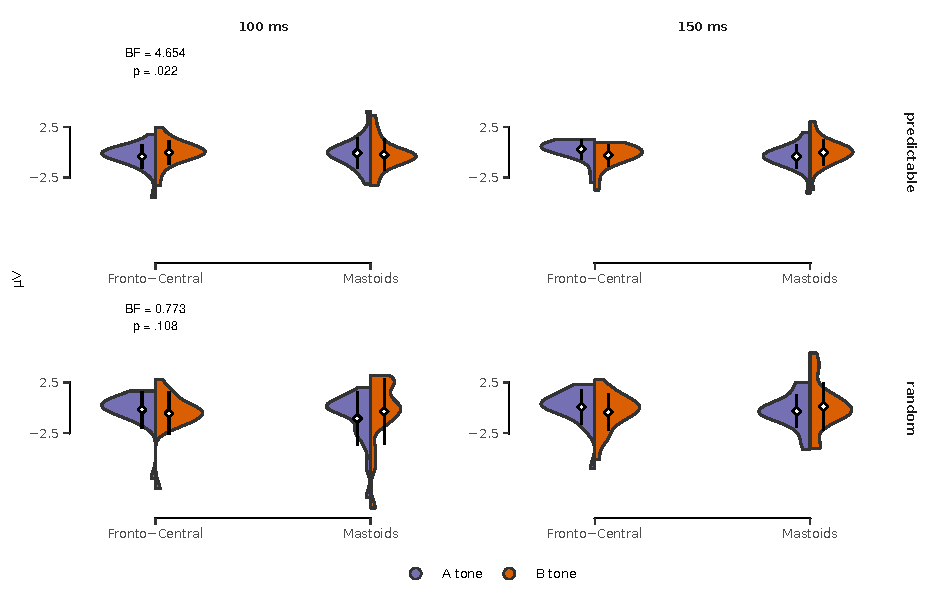
\includegraphics{figures/fig_posthoc.pdf}
\caption{Averaged voltages in the MMN latency window for pooled
frontocentral and mastoid electrodes. Colored areas show sample
probability density function for A tones (green) and B tones (red).
White diamonds indicate estimated population mean, vertical bars
represent 95\%-conficence interval. Only Benjamini-Hochberg-corrected
p-values \(< 0.05\) are shown.}
\end{figure}

\begin{figure}
\hypertarget{fig:fronto2}{%
\centering
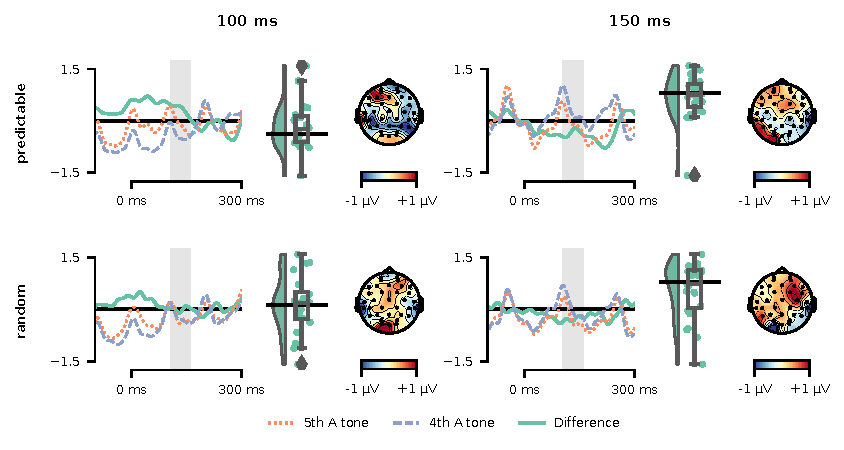
\includegraphics{figures/fig_fronto2.pdf}
\caption{ERP grand averages (pooled FZ, F3, F4, FC1, and FC2 electrode
locations) for an SOA of 100 ms (left) and 150 ms (right), for 4th A
tones (A-A-A-\textbf{A}-X, blue dashed lines) and 5th A tones
(A-A-A-A-\textbf{A}, orange dashed line) and their difference (B - A,
green solid line). Upper panels show ERPs for tones presented in a
predcitable pattern (\emph{predcitable condition}) while lower panels
show ERPs for tones presented in pseudo-random order (\emph{random
condition}). Shaded area marks MMN latency window (110 ms to 160 ms)
used to calculate the distribution of amplitude differences across
particpants (middle of each panel) and the difference of topographic
maps averaged over the same interval (right of each
panel).}\label{fig:fronto2}
}
\end{figure}


  \providecommand{\huxb}[2]{\arrayrulecolor[RGB]{#1}\global\arrayrulewidth=#2pt}
  \providecommand{\huxvb}[2]{\color[RGB]{#1}\vrule width #2pt}
  \providecommand{\huxtpad}[1]{\rule{0pt}{#1}}
  \providecommand{\huxbpad}[1]{\rule[-#1]{0pt}{#1}}

\begin{table}[ht]
\begin{centerbox}
\begin{threeparttable}
\captionsetup{justification=centering,singlelinecheck=off}
\caption{Results of the 2-way ANOVA (condition x stimulus type) for repeated measures. Only fronto included.}
 \setlength{\tabcolsep}{0pt}
\begin{tabular}{l l l l l l l l l}


\hhline{>{\huxb{0, 0, 0}{0.4}}->{\huxb{0, 0, 0}{0.4}}->{\huxb{0, 0, 0}{0.4}}->{\huxb{0, 0, 0}{0.4}}->{\huxb{0, 0, 0}{0.4}}->{\huxb{0, 0, 0}{0.4}}->{\huxb{0, 0, 0}{0.4}}->{\huxb{0, 0, 0}{0.4}}->{\huxb{0, 0, 0}{0.4}}-}
\arrayrulecolor{black}

\multicolumn{1}{!{\huxvb{0, 0, 0}{0}}l!{\huxvb{0, 0, 0}{0}}}{\huxtpad{6pt + 1em}\raggedright \hspace{0pt} \rotatebox{90}{\textbf{}} \hspace{6pt}\huxbpad{6pt}} &
\multicolumn{1}{l!{\huxvb{0, 0, 0}{0}}}{\huxtpad{6pt + 1em}\raggedright \hspace{6pt} \rotatebox{90}{\textbf{}} \hspace{6pt}\huxbpad{6pt}} &
\multicolumn{1}{l!{\huxvb{0, 0, 0}{0}}}{\huxtpad{6pt + 1em}\raggedright \hspace{6pt} \textbf{Effect} \hspace{6pt}\huxbpad{6pt}} &
\multicolumn{1}{r!{\huxvb{0, 0, 0}{0}}}{\huxtpad{6pt + 1em}\raggedleft \hspace{6pt} \textbf{DFn} \hspace{6pt}\huxbpad{6pt}} &
\multicolumn{1}{r!{\huxvb{0, 0, 0}{0}}}{\huxtpad{6pt + 1em}\raggedleft \hspace{6pt} \textbf{DFd} \hspace{6pt}\huxbpad{6pt}} &
\multicolumn{1}{r!{\huxvb{0, 0, 0}{0}}}{\huxtpad{6pt + 1em}\raggedleft \hspace{6pt} \textbf{F} \hspace{6pt}\huxbpad{6pt}} &
\multicolumn{1}{r!{\huxvb{0, 0, 0}{0}}}{\huxtpad{6pt + 1em}\raggedleft \hspace{6pt} \textbf{p} \hspace{6pt}\huxbpad{6pt}} &
\multicolumn{1}{l!{\huxvb{0, 0, 0}{0}}}{\huxtpad{6pt + 1em}\raggedright \hspace{6pt} \textbf{p$<$.05} \hspace{6pt}\huxbpad{6pt}} &
\multicolumn{1}{r!{\huxvb{0, 0, 0}{0}}}{\huxtpad{6pt + 1em}\raggedleft \hspace{6pt} \textbf{ges} \hspace{0pt}\huxbpad{6pt}} \tabularnewline[-0.5pt]


\hhline{>{\huxb{0, 0, 0}{0.4}}->{\huxb{0, 0, 0}{0.4}}->{\huxb{0, 0, 0}{0.4}}->{\huxb{0, 0, 0}{0.4}}->{\huxb{0, 0, 0}{0.4}}->{\huxb{0, 0, 0}{0.4}}->{\huxb{0, 0, 0}{0.4}}->{\huxb{0, 0, 0}{0.4}}->{\huxb{0, 0, 0}{0.4}}-}
\arrayrulecolor{black}

\multicolumn{1}{!{\huxvb{0, 0, 0}{0}}l!{\huxvb{0, 0, 0}{0}}}{} &
\multicolumn{1}{l!{\huxvb{0, 0, 0}{0}}}{} &
\multicolumn{1}{l!{\huxvb{0, 0, 0}{0}}}{\huxtpad{6pt + 1em}\raggedright \hspace{6pt} Condition \hspace{6pt}\huxbpad{6pt}} &
\multicolumn{1}{r!{\huxvb{0, 0, 0}{0}}}{\huxtpad{6pt + 1em}\raggedleft \hspace{6pt} 1 \hspace{6pt}\huxbpad{6pt}} &
\multicolumn{1}{r!{\huxvb{0, 0, 0}{0}}}{\huxtpad{6pt + 1em}\raggedleft \hspace{6pt} 19 \hspace{6pt}\huxbpad{6pt}} &
\multicolumn{1}{r!{\huxvb{0, 0, 0}{0}}}{\huxtpad{6pt + 1em}\raggedleft \hspace{6pt} 0.026 \hspace{6pt}\huxbpad{6pt}} &
\multicolumn{1}{r!{\huxvb{0, 0, 0}{0}}}{\huxtpad{6pt + 1em}\raggedleft \hspace{6pt} .873 \hspace{6pt}\huxbpad{6pt}} &
\multicolumn{1}{l!{\huxvb{0, 0, 0}{0}}}{\huxtpad{6pt + 1em}\raggedright \hspace{6pt}  \hspace{6pt}\huxbpad{6pt}} &
\multicolumn{1}{r!{\huxvb{0, 0, 0}{0}}}{\huxtpad{6pt + 1em}\raggedleft \hspace{6pt} 0.000441 \hspace{0pt}\huxbpad{6pt}} \tabularnewline[-0.5pt]


\hhline{}
\arrayrulecolor{black}

\multicolumn{1}{!{\huxvb{0, 0, 0}{0}}l!{\huxvb{0, 0, 0}{0}}}{} &
\multicolumn{1}{l!{\huxvb{0, 0, 0}{0}}}{} &
\multicolumn{1}{l!{\huxvb{0, 0, 0}{0}}}{\huxtpad{6pt + 1em}\raggedright \hspace{6pt} StimulusType \hspace{6pt}\huxbpad{6pt}} &
\multicolumn{1}{r!{\huxvb{0, 0, 0}{0}}}{\huxtpad{6pt + 1em}\raggedleft \hspace{6pt} 1 \hspace{6pt}\huxbpad{6pt}} &
\multicolumn{1}{r!{\huxvb{0, 0, 0}{0}}}{\huxtpad{6pt + 1em}\raggedleft \hspace{6pt} 19 \hspace{6pt}\huxbpad{6pt}} &
\multicolumn{1}{r!{\huxvb{0, 0, 0}{0}}}{\huxtpad{6pt + 1em}\raggedleft \hspace{6pt} 0.938 \hspace{6pt}\huxbpad{6pt}} &
\multicolumn{1}{r!{\huxvb{0, 0, 0}{0}}}{\huxtpad{6pt + 1em}\raggedleft \hspace{6pt} .345 \hspace{6pt}\huxbpad{6pt}} &
\multicolumn{1}{l!{\huxvb{0, 0, 0}{0}}}{\huxtpad{6pt + 1em}\raggedright \hspace{6pt}  \hspace{6pt}\huxbpad{6pt}} &
\multicolumn{1}{r!{\huxvb{0, 0, 0}{0}}}{\huxtpad{6pt + 1em}\raggedleft \hspace{6pt} 0.002~~~ \hspace{0pt}\huxbpad{6pt}} \tabularnewline[-0.5pt]


\hhline{}
\arrayrulecolor{black}

\multicolumn{1}{!{\huxvb{0, 0, 0}{0}}l!{\huxvb{0, 0, 0}{0}}}{} &
\multicolumn{1}{l!{\huxvb{0, 0, 0}{0}}}{\multirow[c]{-3}{*}[0ex]{\huxtpad{6pt + 1em}\raggedright \hspace{6pt} \rotatebox{90}{Frontal} \hspace{6pt}\huxbpad{6pt}}} &
\multicolumn{1}{l!{\huxvb{0, 0, 0}{0}}}{\huxtpad{6pt + 1em}\raggedright \hspace{6pt} Condition x StimulusType \hspace{6pt}\huxbpad{8pt}} &
\multicolumn{1}{r!{\huxvb{0, 0, 0}{0}}}{\huxtpad{6pt + 1em}\raggedleft \hspace{6pt} 1 \hspace{6pt}\huxbpad{8pt}} &
\multicolumn{1}{r!{\huxvb{0, 0, 0}{0}}}{\huxtpad{6pt + 1em}\raggedleft \hspace{6pt} 19 \hspace{6pt}\huxbpad{8pt}} &
\multicolumn{1}{r!{\huxvb{0, 0, 0}{0}}}{\huxtpad{6pt + 1em}\raggedleft \hspace{6pt} 0.961 \hspace{6pt}\huxbpad{8pt}} &
\multicolumn{1}{r!{\huxvb{0, 0, 0}{0}}}{\huxtpad{6pt + 1em}\raggedleft \hspace{6pt} .339 \hspace{6pt}\huxbpad{8pt}} &
\multicolumn{1}{l!{\huxvb{0, 0, 0}{0}}}{\huxtpad{6pt + 1em}\raggedright \hspace{6pt}  \hspace{6pt}\huxbpad{8pt}} &
\multicolumn{1}{r!{\huxvb{0, 0, 0}{0}}}{\huxtpad{6pt + 1em}\raggedleft \hspace{6pt} 0.002~~~ \hspace{0pt}\huxbpad{8pt}} \tabularnewline[-0.5pt]


\hhline{}
\arrayrulecolor{black}

\multicolumn{1}{!{\huxvb{0, 0, 0}{0}}l!{\huxvb{0, 0, 0}{0}}}{} &
\multicolumn{1}{l!{\huxvb{0, 0, 0}{0}}}{} &
\multicolumn{1}{l!{\huxvb{0, 0, 0}{0}}}{\huxtpad{8pt + 1em}\raggedright \hspace{6pt} Condition \hspace{6pt}\huxbpad{6pt}} &
\multicolumn{1}{r!{\huxvb{0, 0, 0}{0}}}{\huxtpad{8pt + 1em}\raggedleft \hspace{6pt} 1 \hspace{6pt}\huxbpad{6pt}} &
\multicolumn{1}{r!{\huxvb{0, 0, 0}{0}}}{\huxtpad{8pt + 1em}\raggedleft \hspace{6pt} 19 \hspace{6pt}\huxbpad{6pt}} &
\multicolumn{1}{r!{\huxvb{0, 0, 0}{0}}}{\huxtpad{8pt + 1em}\raggedleft \hspace{6pt} 3.59~ \hspace{6pt}\huxbpad{6pt}} &
\multicolumn{1}{r!{\huxvb{0, 0, 0}{0}}}{\huxtpad{8pt + 1em}\raggedleft \hspace{6pt} .073 \hspace{6pt}\huxbpad{6pt}} &
\multicolumn{1}{l!{\huxvb{0, 0, 0}{0}}}{\huxtpad{8pt + 1em}\raggedright \hspace{6pt}  \hspace{6pt}\huxbpad{6pt}} &
\multicolumn{1}{r!{\huxvb{0, 0, 0}{0}}}{\huxtpad{8pt + 1em}\raggedleft \hspace{6pt} 0.063~~~ \hspace{0pt}\huxbpad{6pt}} \tabularnewline[-0.5pt]


\hhline{}
\arrayrulecolor{black}

\multicolumn{1}{!{\huxvb{0, 0, 0}{0}}l!{\huxvb{0, 0, 0}{0}}}{} &
\multicolumn{1}{l!{\huxvb{0, 0, 0}{0}}}{} &
\multicolumn{1}{l!{\huxvb{0, 0, 0}{0}}}{\huxtpad{6pt + 1em}\raggedright \hspace{6pt} StimulusType \hspace{6pt}\huxbpad{6pt}} &
\multicolumn{1}{r!{\huxvb{0, 0, 0}{0}}}{\huxtpad{6pt + 1em}\raggedleft \hspace{6pt} 1 \hspace{6pt}\huxbpad{6pt}} &
\multicolumn{1}{r!{\huxvb{0, 0, 0}{0}}}{\huxtpad{6pt + 1em}\raggedleft \hspace{6pt} 19 \hspace{6pt}\huxbpad{6pt}} &
\multicolumn{1}{r!{\huxvb{0, 0, 0}{0}}}{\huxtpad{6pt + 1em}\raggedleft \hspace{6pt} 1~~~~ \hspace{6pt}\huxbpad{6pt}} &
\multicolumn{1}{r!{\huxvb{0, 0, 0}{0}}}{\huxtpad{6pt + 1em}\raggedleft \hspace{6pt} .330 \hspace{6pt}\huxbpad{6pt}} &
\multicolumn{1}{l!{\huxvb{0, 0, 0}{0}}}{\huxtpad{6pt + 1em}\raggedright \hspace{6pt}  \hspace{6pt}\huxbpad{6pt}} &
\multicolumn{1}{r!{\huxvb{0, 0, 0}{0}}}{\huxtpad{6pt + 1em}\raggedleft \hspace{6pt} 0.003~~~ \hspace{0pt}\huxbpad{6pt}} \tabularnewline[-0.5pt]


\hhline{}
\arrayrulecolor{black}

\multicolumn{1}{!{\huxvb{0, 0, 0}{0}}l!{\huxvb{0, 0, 0}{0}}}{\multirow[c]{-6}{*}[0ex]{\huxtpad{6pt + 1em}\raggedright \hspace{0pt} \rotatebox{90}{100 ms} \hspace{6pt}\huxbpad{6pt}}} &
\multicolumn{1}{l!{\huxvb{0, 0, 0}{0}}}{\multirow[c]{-3}{*}[0ex]{\huxtpad{8pt + 1em}\raggedright \hspace{6pt} \rotatebox{90}{Mastoids} \hspace{6pt}\huxbpad{6pt}}} &
\multicolumn{1}{l!{\huxvb{0, 0, 0}{0}}}{\huxtpad{6pt + 1em}\raggedright \hspace{6pt} Condition x StimulusType \hspace{6pt}\huxbpad{15pt}} &
\multicolumn{1}{r!{\huxvb{0, 0, 0}{0}}}{\huxtpad{6pt + 1em}\raggedleft \hspace{6pt} 1 \hspace{6pt}\huxbpad{15pt}} &
\multicolumn{1}{r!{\huxvb{0, 0, 0}{0}}}{\huxtpad{6pt + 1em}\raggedleft \hspace{6pt} 19 \hspace{6pt}\huxbpad{15pt}} &
\multicolumn{1}{r!{\huxvb{0, 0, 0}{0}}}{\huxtpad{6pt + 1em}\raggedleft \hspace{6pt} 0.822 \hspace{6pt}\huxbpad{15pt}} &
\multicolumn{1}{r!{\huxvb{0, 0, 0}{0}}}{\huxtpad{6pt + 1em}\raggedleft \hspace{6pt} .376 \hspace{6pt}\huxbpad{15pt}} &
\multicolumn{1}{l!{\huxvb{0, 0, 0}{0}}}{\huxtpad{6pt + 1em}\raggedright \hspace{6pt}  \hspace{6pt}\huxbpad{15pt}} &
\multicolumn{1}{r!{\huxvb{0, 0, 0}{0}}}{\huxtpad{6pt + 1em}\raggedleft \hspace{6pt} 0.005~~~ \hspace{0pt}\huxbpad{15pt}} \tabularnewline[-0.5pt]


\hhline{}
\arrayrulecolor{black}

\multicolumn{1}{!{\huxvb{0, 0, 0}{0}}l!{\huxvb{0, 0, 0}{0}}}{} &
\multicolumn{1}{l!{\huxvb{0, 0, 0}{0}}}{} &
\multicolumn{1}{l!{\huxvb{0, 0, 0}{0}}}{\huxtpad{15pt + 1em}\raggedright \hspace{6pt} Condition \hspace{6pt}\huxbpad{6pt}} &
\multicolumn{1}{r!{\huxvb{0, 0, 0}{0}}}{\huxtpad{15pt + 1em}\raggedleft \hspace{6pt} 1 \hspace{6pt}\huxbpad{6pt}} &
\multicolumn{1}{r!{\huxvb{0, 0, 0}{0}}}{\huxtpad{15pt + 1em}\raggedleft \hspace{6pt} 22 \hspace{6pt}\huxbpad{6pt}} &
\multicolumn{1}{r!{\huxvb{0, 0, 0}{0}}}{\huxtpad{15pt + 1em}\raggedleft \hspace{6pt} 0.938 \hspace{6pt}\huxbpad{6pt}} &
\multicolumn{1}{r!{\huxvb{0, 0, 0}{0}}}{\huxtpad{15pt + 1em}\raggedleft \hspace{6pt} .343 \hspace{6pt}\huxbpad{6pt}} &
\multicolumn{1}{l!{\huxvb{0, 0, 0}{0}}}{\huxtpad{15pt + 1em}\raggedright \hspace{6pt}  \hspace{6pt}\huxbpad{6pt}} &
\multicolumn{1}{r!{\huxvb{0, 0, 0}{0}}}{\huxtpad{15pt + 1em}\raggedleft \hspace{6pt} 0.003~~~ \hspace{0pt}\huxbpad{6pt}} \tabularnewline[-0.5pt]


\hhline{}
\arrayrulecolor{black}

\multicolumn{1}{!{\huxvb{0, 0, 0}{0}}l!{\huxvb{0, 0, 0}{0}}}{} &
\multicolumn{1}{l!{\huxvb{0, 0, 0}{0}}}{} &
\multicolumn{1}{l!{\huxvb{0, 0, 0}{0}}}{\huxtpad{6pt + 1em}\raggedright \hspace{6pt} StimulusType \hspace{6pt}\huxbpad{6pt}} &
\multicolumn{1}{r!{\huxvb{0, 0, 0}{0}}}{\huxtpad{6pt + 1em}\raggedleft \hspace{6pt} 1 \hspace{6pt}\huxbpad{6pt}} &
\multicolumn{1}{r!{\huxvb{0, 0, 0}{0}}}{\huxtpad{6pt + 1em}\raggedleft \hspace{6pt} 22 \hspace{6pt}\huxbpad{6pt}} &
\multicolumn{1}{r!{\huxvb{0, 0, 0}{0}}}{\huxtpad{6pt + 1em}\raggedleft \hspace{6pt} 1.6~~ \hspace{6pt}\huxbpad{6pt}} &
\multicolumn{1}{r!{\huxvb{0, 0, 0}{0}}}{\huxtpad{6pt + 1em}\raggedleft \hspace{6pt} .219 \hspace{6pt}\huxbpad{6pt}} &
\multicolumn{1}{l!{\huxvb{0, 0, 0}{0}}}{\huxtpad{6pt + 1em}\raggedright \hspace{6pt}  \hspace{6pt}\huxbpad{6pt}} &
\multicolumn{1}{r!{\huxvb{0, 0, 0}{0}}}{\huxtpad{6pt + 1em}\raggedleft \hspace{6pt} 0.008~~~ \hspace{0pt}\huxbpad{6pt}} \tabularnewline[-0.5pt]


\hhline{}
\arrayrulecolor{black}

\multicolumn{1}{!{\huxvb{0, 0, 0}{0}}l!{\huxvb{0, 0, 0}{0}}}{} &
\multicolumn{1}{l!{\huxvb{0, 0, 0}{0}}}{\multirow[c]{-3}{*}[0ex]{\huxtpad{15pt + 1em}\raggedright \hspace{6pt} \rotatebox{90}{Frontal} \hspace{6pt}\huxbpad{6pt}}} &
\multicolumn{1}{l!{\huxvb{0, 0, 0}{0}}}{\huxtpad{6pt + 1em}\raggedright \hspace{6pt} Condition x StimulusType \hspace{6pt}\huxbpad{8pt}} &
\multicolumn{1}{r!{\huxvb{0, 0, 0}{0}}}{\huxtpad{6pt + 1em}\raggedleft \hspace{6pt} 1 \hspace{6pt}\huxbpad{8pt}} &
\multicolumn{1}{r!{\huxvb{0, 0, 0}{0}}}{\huxtpad{6pt + 1em}\raggedleft \hspace{6pt} 22 \hspace{6pt}\huxbpad{8pt}} &
\multicolumn{1}{r!{\huxvb{0, 0, 0}{0}}}{\huxtpad{6pt + 1em}\raggedleft \hspace{6pt} 0.074 \hspace{6pt}\huxbpad{8pt}} &
\multicolumn{1}{r!{\huxvb{0, 0, 0}{0}}}{\huxtpad{6pt + 1em}\raggedleft \hspace{6pt} .789 \hspace{6pt}\huxbpad{8pt}} &
\multicolumn{1}{l!{\huxvb{0, 0, 0}{0}}}{\huxtpad{6pt + 1em}\raggedright \hspace{6pt}  \hspace{6pt}\huxbpad{8pt}} &
\multicolumn{1}{r!{\huxvb{0, 0, 0}{0}}}{\huxtpad{6pt + 1em}\raggedleft \hspace{6pt} 0.000258 \hspace{0pt}\huxbpad{8pt}} \tabularnewline[-0.5pt]


\hhline{}
\arrayrulecolor{black}

\multicolumn{1}{!{\huxvb{0, 0, 0}{0}}l!{\huxvb{0, 0, 0}{0}}}{} &
\multicolumn{1}{l!{\huxvb{0, 0, 0}{0}}}{} &
\multicolumn{1}{l!{\huxvb{0, 0, 0}{0}}}{\huxtpad{8pt + 1em}\raggedright \hspace{6pt} Condition \hspace{6pt}\huxbpad{6pt}} &
\multicolumn{1}{r!{\huxvb{0, 0, 0}{0}}}{\huxtpad{8pt + 1em}\raggedleft \hspace{6pt} 1 \hspace{6pt}\huxbpad{6pt}} &
\multicolumn{1}{r!{\huxvb{0, 0, 0}{0}}}{\huxtpad{8pt + 1em}\raggedleft \hspace{6pt} 22 \hspace{6pt}\huxbpad{6pt}} &
\multicolumn{1}{r!{\huxvb{0, 0, 0}{0}}}{\huxtpad{8pt + 1em}\raggedleft \hspace{6pt} 0.875 \hspace{6pt}\huxbpad{6pt}} &
\multicolumn{1}{r!{\huxvb{0, 0, 0}{0}}}{\huxtpad{8pt + 1em}\raggedleft \hspace{6pt} .360 \hspace{6pt}\huxbpad{6pt}} &
\multicolumn{1}{l!{\huxvb{0, 0, 0}{0}}}{\huxtpad{8pt + 1em}\raggedright \hspace{6pt}  \hspace{6pt}\huxbpad{6pt}} &
\multicolumn{1}{r!{\huxvb{0, 0, 0}{0}}}{\huxtpad{8pt + 1em}\raggedleft \hspace{6pt} 0.005~~~ \hspace{0pt}\huxbpad{6pt}} \tabularnewline[-0.5pt]


\hhline{}
\arrayrulecolor{black}

\multicolumn{1}{!{\huxvb{0, 0, 0}{0}}l!{\huxvb{0, 0, 0}{0}}}{} &
\multicolumn{1}{l!{\huxvb{0, 0, 0}{0}}}{} &
\multicolumn{1}{l!{\huxvb{0, 0, 0}{0}}}{\huxtpad{6pt + 1em}\raggedright \hspace{6pt} StimulusType \hspace{6pt}\huxbpad{6pt}} &
\multicolumn{1}{r!{\huxvb{0, 0, 0}{0}}}{\huxtpad{6pt + 1em}\raggedleft \hspace{6pt} 1 \hspace{6pt}\huxbpad{6pt}} &
\multicolumn{1}{r!{\huxvb{0, 0, 0}{0}}}{\huxtpad{6pt + 1em}\raggedleft \hspace{6pt} 22 \hspace{6pt}\huxbpad{6pt}} &
\multicolumn{1}{r!{\huxvb{0, 0, 0}{0}}}{\huxtpad{6pt + 1em}\raggedleft \hspace{6pt} 2.8~~ \hspace{6pt}\huxbpad{6pt}} &
\multicolumn{1}{r!{\huxvb{0, 0, 0}{0}}}{\huxtpad{6pt + 1em}\raggedleft \hspace{6pt} .109 \hspace{6pt}\huxbpad{6pt}} &
\multicolumn{1}{l!{\huxvb{0, 0, 0}{0}}}{\huxtpad{6pt + 1em}\raggedright \hspace{6pt}  \hspace{6pt}\huxbpad{6pt}} &
\multicolumn{1}{r!{\huxvb{0, 0, 0}{0}}}{\huxtpad{6pt + 1em}\raggedleft \hspace{6pt} 0.009~~~ \hspace{0pt}\huxbpad{6pt}} \tabularnewline[-0.5pt]


\hhline{}
\arrayrulecolor{black}

\multicolumn{1}{!{\huxvb{0, 0, 0}{0}}l!{\huxvb{0, 0, 0}{0}}}{\multirow[c]{-6}{*}[0ex]{\huxtpad{15pt + 1em}\raggedright \hspace{0pt} \rotatebox{90}{150 ms} \hspace{6pt}\huxbpad{6pt}}} &
\multicolumn{1}{l!{\huxvb{0, 0, 0}{0}}}{\multirow[c]{-3}{*}[0ex]{\huxtpad{8pt + 1em}\raggedright \hspace{6pt} \rotatebox{90}{Mastoids} \hspace{6pt}\huxbpad{6pt}}} &
\multicolumn{1}{l!{\huxvb{0, 0, 0}{0}}}{\huxtpad{6pt + 1em}\raggedright \hspace{6pt} Condition x StimulusType \hspace{6pt}\huxbpad{6pt}} &
\multicolumn{1}{r!{\huxvb{0, 0, 0}{0}}}{\huxtpad{6pt + 1em}\raggedleft \hspace{6pt} 1 \hspace{6pt}\huxbpad{6pt}} &
\multicolumn{1}{r!{\huxvb{0, 0, 0}{0}}}{\huxtpad{6pt + 1em}\raggedleft \hspace{6pt} 22 \hspace{6pt}\huxbpad{6pt}} &
\multicolumn{1}{r!{\huxvb{0, 0, 0}{0}}}{\huxtpad{6pt + 1em}\raggedleft \hspace{6pt} 0.93~ \hspace{6pt}\huxbpad{6pt}} &
\multicolumn{1}{r!{\huxvb{0, 0, 0}{0}}}{\huxtpad{6pt + 1em}\raggedleft \hspace{6pt} .345 \hspace{6pt}\huxbpad{6pt}} &
\multicolumn{1}{l!{\huxvb{0, 0, 0}{0}}}{\huxtpad{6pt + 1em}\raggedright \hspace{6pt}  \hspace{6pt}\huxbpad{6pt}} &
\multicolumn{1}{r!{\huxvb{0, 0, 0}{0}}}{\huxtpad{6pt + 1em}\raggedleft \hspace{6pt} 0.003~~~ \hspace{0pt}\huxbpad{6pt}} \tabularnewline[-0.5pt]


\hhline{>{\huxb{0, 0, 0}{0.4}}->{\huxb{0, 0, 0}{0.4}}->{\huxb{0, 0, 0}{0.4}}->{\huxb{0, 0, 0}{0.4}}->{\huxb{0, 0, 0}{0.4}}->{\huxb{0, 0, 0}{0.4}}->{\huxb{0, 0, 0}{0.4}}->{\huxb{0, 0, 0}{0.4}}->{\huxb{0, 0, 0}{0.4}}-}
\arrayrulecolor{black}
\end{tabular}
\end{threeparttable}\par\end{centerbox}

\end{table}



\begin{figure}
\hypertarget{fig:rel}{%
\centering
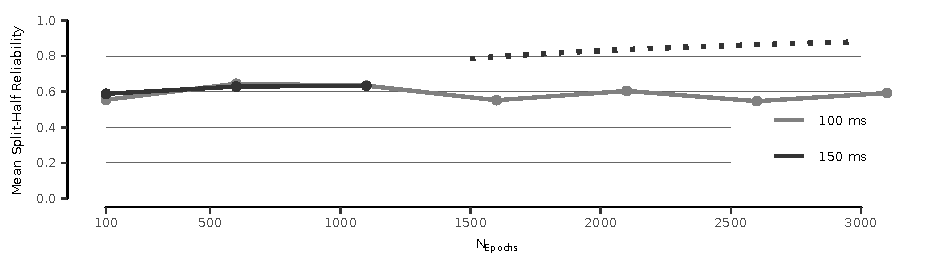
\includegraphics{figures/fig_subsample_rel.pdf}
\caption{Average split-half reliabilities for A and B tones in random
and predictable contexts.. Negative values might be interpreted as low
or no reliability (\textbf{cronbachNoteNegativeReliabilities1954?}).
Thin lines in the 150 ms condition indicate extrapolation using the
Spearman-Brown formula.}\label{fig:rel}
}
\end{figure}

Average split-half reliabilities (Fig.~\ref{fig:rel}) demonstrate that
reliability can be characterized as a function of epoch number. Whereas
a high number of epochs provided reasonable reliability, particularly
small samples resulted in highly unreliable estimates. This observation
might serve as a plausible explanation for aforementioned inconclusive
result insofar as epoch numbers for B tones (\(N_{avg} = 364.4\)) could
be inadequately low to obtain a reliable estimate. In comparison,
including all B tones (instead of only tones that were part of a
five-tone pattern and akin to E. S. Sussman \& Gumenyuk (2005)), on
average led to an eightfold increase in epoch numbers
(\(N_{avg} = 2919.8\)). Interestingly, statistical comparison for such
an extended sample was no longer inconclusive but indicated strong
evidence in favor of an effect (\(t(19) = 3.31\), \(p = .004\),
\(CI_{.95} = [0.20,0.88], BF_{10} = 11.92\)).

\newpage

\hypertarget{discussion}{%
\section{Discussion}\label{discussion}}

For the 150 presentation, extreme evidence for an MMN and very strong
evidence for an accopying polarity reversal at the mastoids was found in
the \emph{predcitable} condition, that is, when tones were presented in
a repeated five-tone pattern. When tones were presented in random order,
strong evidence was foun{[}{[}anova\_02\_100\_posthoc{]}{]}
anova\_02\_100\_posthoc.texd for an MMN but Bayes factors suggested
inconclusive evidence for mastoids. In light of the resuts by E. S.
Sussman \& Gumenyuk (2005), we would

% \usepackage{booktabs}


\begin{table}
\centering
\begin{tabular*}{\textwidth}{lcllc} 
\toprule
                                                                                                                & \multicolumn{2}{c}{Predictable Context}               & Difference Wave                                                \\ 
\cmidrule(lr){2-3}\cmidrule(lr){4-4}
\multicolumn{1}{c}{}                                                                         & $\mathcal{H_1}: B_{5th}<A_{4th}$     & $\mathcal{H_1}: A_{5th}<A_{4th}$     & \multicolumn{1}{c}{$\mathcal{H_1}: \Lambda_{rand} \neq \Lambda_{pred}$ }  \\ 
%\cmidrule(lr){2-2}\cmidrule(lr){3-3}\cmidrule(lr){4-4}\cmidrule(lr){5-5}
\midrule
\multicolumn{5}{l}{\textbf{\textit{Expected Pattern Secondary Hypotheses}}}  \\
\hspace{3mm}\textit{Only pattern regularities used}                                                                                         & \multicolumn{1}{c}{×} & \multicolumn{1}{c}{✓} & \multicolumn{1}{c}{✓}\\
\hspace{3mm}\textit{Only Proportional regularities used}                                                                                    & \multicolumn{1}{c}{✓} & \multicolumn{1}{c}{×} & \multicolumn{1}{c}{×}\\
\hspace{3mm}\textit{Concurrent usage}                                								         & \multicolumn{1}{c}{✓} & \multicolumn{1}{c}{✓} & \multicolumn{1}{c}{}\\
\multicolumn{5}{l}{\textbf{\textit{Results}}}  \\
\hspace{3mm}100 ms SOA                                                                                                                      & \multicolumn{1}{c}{n.s.}                 & \multicolumn{1}{c}{n.s.}                    & \multicolumn{1}{c}{✓}                                      \\
\hspace{3mm}150 ms SOA                                                                                                                      & \multicolumn{1}{c}{✓}                      & \multicolumn{1}{c}{n.s.}                    & \multicolumn{1}{c}{n.s.}                                    \\
\bottomrule
\end{tabular*}
 \begin{tablenotes}
      \small
      \item ✓: $\mathcal{H_1}$ is true / $\mathcal{H_0}$ rejected, ×: $\mathcal{H_0}$ is true, \textit{inc}: inconclusive results \~{}: no explicit expectation
    \end{tablenotes}
\end{table}


We found strong evidence for an MMN in the 150 ms delivery rate
condition when comparing standards and deviants, regardless of the type
of presentation (predictable vs.~random). This finding is incompatible
with the results and intepretation by (E. S. Sussman \& Gumenyuk, 2005)
but suggests that \emph{pattern regularities} do not inform prediction.
Furthermore, no convincing evidence for an MMN was found when comparing
the 4th standard to the 5th standard in predictable condition.

For the 150 ms , significant MMN componets were found regardless of
presentation

Lorem ipsum dolor sit amet, consectetur adipiscing elit. Donec id cursus
velit, non egestas quam. Aliquam rutrum eget sem ut aliquet. Etiam
euismod purus et gravida volutpat. Suspendisse consequat ipsum nibh,
vitae convallis dolor efficitur a. Suspendisse vehicula erat posuere
velit fermentum viverra. Proin sapien urna, iaculis ut ultricies ac,
auctor eu est. Nunc ornare pharetra finibus. Morbi finibus, ipsum non
accumsan cursus, metus nisl egestas leo, et aliquam nisi leo quis diam.
Quisque id diam non risus elementum convallis. Duis non nisl at nisl
imperdiet vestibulum. Suspendisse efficitur porttitor nulla a vehicula.
Interdum et malesuada fames ac ante ipsum primis in faucibus. Praesent
tempor urna in orci congue, non euismod eros volutpat. Integer
ullamcorper auctor libero, in laoreet nulla hendrerit ultrices.

Proin malesuada nisi et luctus volutpat. Nam ac posuere enim. Proin nec
augue tincidunt felis ullamcorper luctus ac sit amet mi. Maecenas
aliquam leo quis enim gravida maximus. Sed nec pellentesque magna.
Vivamus et purus lacus. Donec maximus purus at fermentum efficitur.
Phasellus auctor orci sem, eu sollicitudin eros pretium a.

In maximus libero at purus lobortis efficitur. Aliquam nec sapien
consequat, lobortis lorem id, luctus velit. Pellentesque habitant morbi
tristique senectus et netus et malesuada fames ac turpis egestas.
Vestibulum dictum ipsum eu nunc maximus, quis ornare augue tincidunt.
Nam leo purus, mollis quis nunc sed, sagittis tempus orci. In
condimentum et neque ut laoreet. Curabitur accumsan ligula eu libero
iaculis ullamcorper. Interdum et malesuada fames ac ante ipsum primis in
faucibus. Nullam iaculis tellus risus, vitae dapibus augue commodo a.
Sed ante dolor, fermentum at lectus id, pulvinar viverra elit. Aenean
tincidunt mollis imperdiet.

Nulla id molestie neque, vitae vulputate velit. Fusce a velit imperdiet
felis porttitor scelerisque. Nam tempus tincidunt elit, id finibus
tortor tristique non. Ut imperdiet finibus mauris, in fringilla mauris
blandit auctor. Etiam volutpat quam et feugiat elementum. Duis finibus
fermentum condimentum. Donec sollicitudin molestie dolor. Cras convallis
lorem orci, ut sagittis risus rutrum eget. Donec vel lobortis justo.

Pellentesque habitant morbi tristique senectus et netus et malesuada
fames ac turpis egestas. Proin non leo vehicula, congue elit faucibus,
tincidunt diam. Sed euismod vulputate mauris. Duis dapibus faucibus
arcu, ut vehicula tellus blandit eu. Duis erat magna, cursus quis urna
nec, placerat blandit lectus. Maecenas dolor quam, pharetra a urna eu,
mollis iaculis dolor. Aliquam maximus ante eget felis faucibus porta.
Cras semper felis non tellus rutrum tempus. Morbi quam metus, volutpat
nec aliquam at, interdum a nibh. Sed hendrerit purus tempor ex placerat,
ut fringilla nulla molestie. Nullam vitae sem non purus lobortis
fermentum. Quisque ligula tellus, ullamcorper sit amet consectetur quis,
fermentum ac mi. Nunc pretium mollis dictum.

In the context of classcial test theory, this method relates the length
of a test (or \emph{experiment}) to the number of items (or
\emph{trials}). The first derivitve of the Spearman-Brown function is
monotonically decreasing, leading to two different observation: i)
Adding additional epochs (extending the test length by an absolute value
in classcial test theory terms) has a large effect when the number of
already present epochs is low, but has only little effect when already
dealing with large numbers of epochs and ii) SOA and thus effect sized
have a larger impact when epoch numbers are small compared to high epoch
numbers. Graphed values also show that reliabilities for the 100 ms
stimulation rate are considerably lower than for an SOA of 150 ms and
that reliabilities are very low when using a relatively small number of
epochs. There is no generally accepted rule as to the level above which
the coefficient can be considered acceptable. Rather, reliabiliy should
be evaluated based on the purpose of a study considering the
cost-benefit trade-off (\textbf{nunnallyPsychometricTheory1994?}). As
laid out, inreased realibility comes at overproportionate cost, in that
collecting more samples will not increase ralibility by the same factor.
That said, many published articles deem reliability coefficients above
.7 or .8 \enquote{acceptable} (\textbf{lanceSourcesFourCommonly2006?}).
\newpage \# References

\hypertarget{refs}{}
\begin{CSLReferences}{1}{0}
\leavevmode\hypertarget{ref-ablinFasterIndependentComponent2018}{}%
Ablin, P., Cardoso, J.-F., \& Gramfort, A. (2018). Faster independent
component analysis by preconditioning with Hessian approximations.
\emph{IEEE Transactions on Signal Processing}, \emph{66}(15),
4040--4049. \url{https://doi.org/10.1109/TSP.2018.2844203}

\leavevmode\hypertarget{ref-ablinFasterICAOrthogonal2017}{}%
Ablin, P., Cardoso, J.-F., \& Gramfort, A. (2017). Faster ICA under
orthogonal constraint. \emph{arXiv:1711.10873 {[}Stat{]}}.
\url{http://arxiv.org/abs/1711.10873}

\leavevmode\hypertarget{ref-alainBrainIndicesAutomatic1994}{}%
Alain, C., Woods, D. L., \& Ogawa, K. H. (1994). Brain indices of
automatic pattern processing: \emph{NeuroReport}, \emph{6}(1), 140--144.
\url{https://doi.org/10.1097/00001756-199412300-00036}

\leavevmode\hypertarget{ref-bigdely-shamloPREPPipelineStandardized2015}{}%
Bigdely-Shamlo, N., Mullen, T., Kothe, C., Su, K.-M., \& Robbins, K. A.
(2015). The PREP pipeline: standardized preprocessing for large-scale
EEG analysis. \emph{Frontiers in Neuroinformatics}, \emph{9}.
\url{https://doi.org/10.3389/fninf.2015.00016}

\leavevmode\hypertarget{ref-decheveigneZapLineSimpleEffective2020}{}%
de Cheveigné, A. (2020). ZapLine: A simple and effective method to
remove power line artifacts. \emph{NeuroImage}, \emph{207}, 116356.
\url{https://doi.org/10.1016/j.neuroimage.2019.116356}

\leavevmode\hypertarget{ref-decheveigneFiltersWhenWhy2019}{}%
de Cheveigné, A., \& Nelken, I. (2019). Filters: When, Why, and How
(Not) to Use Them. \emph{Neuron}, \emph{102}(2), 280--293.
\url{https://doi.org/10.1016/j.neuron.2019.02.039}

\leavevmode\hypertarget{ref-delormeEEGLABOpenSource2004}{}%
Delorme, A., \& Makeig, S. (2004). EEGLAB: an open source toolbox for
analysis of single-trial EEG dynamics including independent component
analysis. \emph{Journal of Neuroscience Methods}, \emph{134}(1), 9--21.
\url{https://doi.org/10.1016/j.jneumeth.2003.10.009}

\leavevmode\hypertarget{ref-gramfortMEGEEGData2013}{}%
Gramfort, A. (2013). MEG and EEG data analysis with MNE-Python.
\emph{Frontiers in Neuroscience}, \emph{7}.
\url{https://doi.org/10.3389/fnins.2013.00267}

\leavevmode\hypertarget{ref-mullenRealtimeNeuroimagingCognitive2015}{}%
Mullen, T. R., Kothe, C. A. E., Chi, Y. M., Ojeda, A., Kerth, T.,
Makeig, S., Jung, T.-P., \& Cauwenberghs, G. (2015). Real-time
neuroimaging and cognitive monitoring using wearable dry EEG. \emph{IEEE
Transactions on Biomedical Engineering}, \emph{62}(11), 2553--2567.
\url{https://doi.org/10.1109/TBME.2015.2481482}

\leavevmode\hypertarget{ref-nordbyEventRelatedPotentialsBreaks1988}{}%
Nordby, H., Roth, W. T., \& Pfefferbaum, A. (1988). Event-Related
Potentials to Breaks in Sequences of Alternating Pitches or
Interstimulus Intervals. \emph{Psychophysiology}, \emph{25}(3),
262--268. \url{https://doi.org/10.1111/j.1469-8986.1988.tb01239.x}

\leavevmode\hypertarget{ref-paavilainenMismatchnegativityMMNComponent2013}{}%
Paavilainen, P. (2013). The mismatch-negativity (MMN) component of the
auditory event-related potential to violations of abstract regularities:
A review. \emph{International Journal of Psychophysiology},
\emph{88}(2), 109--123.
\url{https://doi.org/10.1016/j.ijpsycho.2013.03.015}

\leavevmode\hypertarget{ref-perrinSphericalSplinesScalp1989}{}%
Perrin, F., Pernier, J., Bertrand, O., \& Echallier, J. F. (1989).
Spherical splines for scalp potential and current density mapping.
\emph{Electroencephalography and Clinical Neurophysiology},
\emph{72}(2), 184--187.
\url{https://doi.org/10.1016/0013-4694(89)90180-6}

\leavevmode\hypertarget{ref-pion-tonachiniICLabelAutomatedElectroencephalographic2019}{}%
Pion-Tonachini, L., Kreutz-Delgado, K., \& Makeig, S. (2019). ICLabel:
An automated electroencephalographic independent component classifier,
dataset, and website. \emph{NeuroImage}, \emph{198}, 181--197.
\url{https://doi.org/10.1016/j.neuroimage.2019.05.026}

\leavevmode\hypertarget{ref-saarinenRepresentationAbstractAttributes1992}{}%
Saarinen, J., Paavilainen, P., Schöger, E., Tervaniemi, M., \& Näätänen,
R. (1992). Representation of abstract attributes of auditory stimuli in
the human brain: \emph{NeuroReport}, \emph{3}(12), 1149--1151.
\url{https://doi.org/10.1097/00001756-199212000-00030}

\leavevmode\hypertarget{ref-schrogerPreattentivePeriodicityDetection1996}{}%
Schröger, E., Tervaniemi, M., Wolff, C., \& Näätänen, R. N. (1996).
Preattentive periodicity detection in auditory patterns as governed by
time and intensity information. \emph{Cognitive Brain Research},
\emph{4}(2), 145--148.
\url{https://doi.org/10.1016/0926-6410(96)00023-7}

\leavevmode\hypertarget{ref-sussmanPredictabilityStimulusDeviance1998}{}%
Sussman, E., Ritter, W., \& Vaughan, H. G. (1998). Predictability of
stimulus deviance and the mismatch negativity: \emph{NeuroReport},
\emph{9}(18), 4167--4170.
\url{https://doi.org/10.1097/00001756-199812210-00031}

\leavevmode\hypertarget{ref-sussmanOrganizationSequentialSounds2005}{}%
Sussman, E. S., \& Gumenyuk, V. (2005). Organization of sequential
sounds in auditory memory: \emph{NeuroReport}, \emph{16}(13),
1519--1523. \url{https://doi.org/10.1097/01.wnr.0000177002.35193.4c}

\leavevmode\hypertarget{ref-widmannDigitalFilterDesign2015}{}%
Widmann, A., Schröger, E., \& Maess, B. (2015). Digital filter design
for electrophysiological data -- a practical approach. \emph{Journal of
Neuroscience Methods}, \emph{250}, 34--46.
\url{https://doi.org/10.1016/j.jneumeth.2014.08.002}

\leavevmode\hypertarget{ref-winklerInterpretingMismatchNegativity2007}{}%
Winkler, István. (2007). Interpreting the Mismatch Negativity.
\emph{Journal of Psychophysiology}, \emph{21}(3-4), 147--163.
\url{https://doi.org/10.1027/0269-8803.21.34.147}

\leavevmode\hypertarget{ref-winklerInfluenceHighpassFiltering2015}{}%
Winkler, Irene, Debener, S., Müller, K.-R., \& Tangermann, M. (2015). On
the influence of high-pass filtering on ICA-based artifact reduction in
EEG-ERP. \emph{2015 37th Annual International Conference of the IEEE
Engineering in Medicine and Biology Society (EMBC)}, 4101--4105.
\url{https://doi.org/10.1109/EMBC.2015.7319296}

\end{CSLReferences}

\end{document}
